% Template for PLoS
% Version 3.4 January 2017
%
% % % % % % % % % % % % % % % % % % % % % %
%
% -- IMPORTANT NOTE
%
% This template contains comments intended 
% to minimize problems and delays during our production 
% process. Please follow the template instructions
% whenever possible.
%
% % % % % % % % % % % % % % % % % % % % % % % 
%
% Once your paper is accepted for publication, 
% PLEASE REMOVE ALL TRACKED CHANGES in this file 
% and leave only the final text of your manuscript. 
% PLOS recommends the use of latexdiff to track changes during review, as this will help to maintain a clean tex file.
% Visit https://www.ctan.org/pkg/latexdiff?lang=en for info or contact us at latex@plos.org.
%
%
% There are no restrictions on package use within the LaTeX files except that 
% no packages listed in the template may be deleted.
%
% Please do not include colors or graphics in the text.
%
% The manuscript LaTeX source should be contained within a single file (do not use \input, \externaldocument, or similar commands).
%
% % % % % % % % % % % % % % % % % % % % % % %
%
% -- FIGURES AND TABLES
%
% Please include tables/figure captions directly after the paragraph where they are first cited in the text.
%
% DO NOT INCLUDE GRAPHICS IN YOUR MANUSCRIPT
% - Figures should be uploaded separately from your manuscript file. 
% - Figures generated using LaTeX should be extracted and removed from the PDF before submission. 
% - Figures containing multiple panels/subfigures must be combined into one image file before submission.
% For figure citations, please use "Fig" instead of "Figure".
% See http://journals.plos.org/plosone/s/figures for PLOS figure guidelines.
%
% Tables should be cell-based and may not contain:
% - spacing/line breaks within cells to alter layout or alignment
% - do not nest tabular environments (no tabular environments within tabular environments)
% - no graphics or colored text (cell background color/shading OK)
% See http://journals.plos.org/plosone/s/tables for table guidelines.
%
% For tables that exceed the width of the text column, use the adjustwidth environment as illustrated in the example table in text below.
%
% % % % % % % % % % % % % % % % % % % % % % % %
%
% -- EQUATIONS, MATH SYMBOLS, SUBSCRIPTS, AND SUPERSCRIPTS
%
% IMPORTANT
% Below are a few tips to help format your equations and other special characters according to our specifications. For more tips to help reduce the possibility of formatting errors during conversion, please see our LaTeX guidelines at http://journals.plos.org/plosone/s/latex
%
% For inline equations, please be sure to include all portions of an equation in the math environment.  For example, x$^2$ is incorrect; this should be formatted as $x^2$ (or $\mathrm{x}^2$ if the romanized font is desired).
%
% Do not include text that is not math in the math environment. For example, CO2 should be written as CO\textsubscript{2} instead of CO$_2$.
%
% Please add line breaks to long display equations when possible in order to fit size of the column. 
%
% For inline equations, please do not include punctuation (commas, etc) within the math environment unless this is part of the equation.
%
% When adding superscript or subscripts outside of brackets/braces, please group using {}.  For example, change "[U(D,E,\gamma)]^2" to "{[U(D,E,\gamma)]}^2". 
%
% Do not use \cal for caligraphic font.  Instead, use \mathcal{}
%
% % % % % % % % % % % % % % % % % % % % % % % % 
%
% Please contact latex@plos.org with any questions.
%
% % % % % % % % % % % % % % % % % % % % % % % %

\documentclass[10pt]{article}
\usepackage[top=0.85in,left=2.75in,footskip=0.75in]{geometry}

% amsmath and amssymb packages, useful for mathematical formulas and symbols
\usepackage{amsmath,amssymb}

% Use adjustwidth environment to exceed column width (see example table in text)
\usepackage{changepage}

% Use Unicode characters when possible
\usepackage[utf8x]{inputenc}

% textcomp package and marvosym package for additional characters
\usepackage{textcomp,marvosym}

% cite package, to clean up citations in the main text. Do not remove.
\usepackage{cite}

% Use nameref to cite supporting information files (see Supporting Information section for more info)
\usepackage{nameref,hyperref}

% line numbers
\usepackage[right]{lineno}

% ligatures disabled
\usepackage{microtype}
\DisableLigatures[f]{encoding = *, family = * }

% color can be used to apply background shading to table cells only
\usepackage[table]{xcolor}

% array package and thick rules for tables
\usepackage{array}

\usepackage{amssymb}
%\usepackage{check-short}
\usepackage{overpic}
\usepackage{multirow}
\usepackage{enumerate}
\usepackage{siunitx}
\usepackage{tikz,pgfplots}
%\usepackage{here}
\usepackage{endfloat}
\renewcommand{\floatpagefraction}{0.1}

% create "+" rule type for thick vertical lines
\newcolumntype{+}{!{\vrule width 2pt}}

% create \thickcline for thick horizontal lines of variable length
\newlength\savedwidth
\newcommand\thickcline[1]{%
  \noalign{\global\savedwidth\arrayrulewidth\global\arrayrulewidth 2pt}%
  \cline{#1}%
  \noalign{\vskip\arrayrulewidth}%
  \noalign{\global\arrayrulewidth\savedwidth}%
}

% \thickhline command for thick horizontal lines that span the table
\newcommand\thickhline{\noalign{\global\savedwidth\arrayrulewidth\global\arrayrulewidth 2pt}%
\hline
\noalign{\global\arrayrulewidth\savedwidth}}


% Remove comment for double spacing
%\usepackage{setspace} 
%\doublespacing

% Text layout
\raggedright
\setlength{\parindent}{0.5cm}
\textwidth 5.25in 
\textheight 8.75in

% Bold the 'Figure #' in the caption and separate it from the title/caption with a period
% Captions will be left justified
\usepackage[aboveskip=1pt,labelfont=bf,labelsep=period,justification=raggedright,singlelinecheck=off]{caption}
\renewcommand{\figurename}{Fig}

% Use the PLoS provided BiBTeX style
\bibliographystyle{plos2015}

% Remove brackets from numbering in List of References
\makeatletter
\renewcommand{\@biblabel}[1]{\quad#1.}
\makeatother

% Leave date blank
\date{}

% Header and Footer with logo
\usepackage{lastpage,fancyhdr,graphicx}
\usepackage{epstopdf}
\pagestyle{myheadings}
\pagestyle{fancy}
\fancyhf{}
\setlength{\headheight}{27.023pt}
\lhead{
\includegraphics[width=2.0in]{PLOS-submission.eps}}
\rfoot{\thepage/\pageref{LastPage}}
\renewcommand{\footrule}{\hrule height 2pt \vspace{2mm}}
\fancyheadoffset[L]{2.25in}
\fancyfootoffset[L]{2.25in}
\lfoot{\sf PLOS}

%% Include all macros below

%\newcommand{\lorem}{{\bf LOREM}}
%\newcommand{\ipsum}{{\bf IPSUM}}

%% END MACROS SECTION


\begin{document}
\vspace*{0.2in}

% Title must be 250 characters or less.
\begin{flushleft}
{\Large
\textbf\newline{Accuracy of perfusion measurements in coupled systems} % Please use "sentence case" for title and headings (capitalize only the first word in a title (or heading), the first word in a subtitle (or subheading), and any proper nouns).
}
\newline
% Insert author names, affiliations and corresponding author email (do not include titles, positions, or degrees).
\\
Constantin Sandmann\textsuperscript{1},
Erik A. Hanson\textsuperscript{2},
Alexander Malyshev\textsuperscript{2},
Arvid Lundervold\textsuperscript{3,4},
Jan Modersitzki\textsuperscript{1},
Erlend Hodneland\textsuperscript{5,6*}
\\
\bigskip
\textbf{1} Institute of Mathematics and Image Computing, University of L\"ubeck, Germany
\\
\textbf{2} Department of Mathematics, University of Bergen, Norway
\\
\textbf{3} Department of Biomedicine, University of Bergen, Norway
\\
\textbf{4} Department of Radiology, Haukeland University Hospital, Norway
\\
\textbf{5} Christian Michelsen Research, Bergen, Norway
\\
\textbf{6} MedViz Research Cluster, University of Bergen, Norway
\\
\bigskip

% Insert additional author notes using the symbols described below. Insert symbol callouts after author names as necessary.
% 
% Remove or comment out the author notes below if they aren't used.
%
% Primary Equal Contribution Note
%\Yinyang These authors contributed equally to this work.

% Additional Equal Contribution Note
% Also use this double-dagger symbol for special authorship notes, such as senior authorship.
%\ddag These authors also contributed equally to this work.

% Current address notes
%\textcurrency Current Address: Dept/Program/Center, Institution Name, City, State, Country % change symbol to "\textcurrency a" if more than one current address note
% \textcurrency b Insert second current address 
% \textcurrency c Insert third current address

% Deceased author note
%\dag Deceased

% Group/Consortium Author Note
%\textpilcrow Membership list can be found in the Acknowledgments section.

% Use the asterisk to denote corresponding authorship and provide email address in note below.
* erlend.hodneland@cmr.no

\end{flushleft}

\newcommand{\missingsource}{\textcolor{red}{[?]}}
\newlength{\fwd}
\newlength{\fht}

% Please keep the abstract below 300 words
\section{Abstract}
One-compartment models are widely used to quantify hemodynamic parameters such as perfusion, blood volume and mean transit time. These parameters are routinely used for clinical diagnosis and monitoring of disease development and are thus of high relevance. However, it is known that common estimation techniques are discretization dependent and values can be erroneous. In this paper we present a new model that enables a systematic quantification of discretization errors. Specifically, we introduce a continuous flow model for tracer propagation within the capillary tissue, used to analyze state-of-the-art one-compartment models. We demonstrate that one-compartment models are capable of recovering perfusion accurately when applied to only one compartment, i.e. the whole region of interest. However, substantial overestimation of perfusion occurs when applied to fractions of a compartment. We further provide values of the estimated overestimation for various discretization levels, and also show that overestimation can be observed in real-life applications. Common practice of using compartment models for fractions of tissue violates model assumptions and careful interpretation is needed when using the computed values for diagnosis and treatment planning.


% Please keep the Author Summary between 150 and 200 words
% Use first person. PLOS ONE authors please skip this step. 
% Author Summary not valid for PLOS ONE submissions.   
%\section{Author summary}
%Lorem ipsum dolor sit amet, consectetur adipiscing elit. Curabitur eget porta erat. Morbi consectetur est vel gravida pretium. Suspendisse ut dui eu ante cursus gravida non sed sem. Nullam sapien tellus, commodo id velit id, eleifend volutpat quam. Phasellus mauris velit, dapibus finibus elementum vel, pulvinar non tellus. Nunc pellentesque pretium diam, quis maximus dolor faucibus id. Nunc convallis sodales ante, ut ullamcorper est egestas vitae. Nam sit amet enim ultrices, ultrices elit pulvinar, volutpat risus.

\linenumbers

% Use "Eq" instead of "Equation" for equation citations.
\section{Introduction}
Quantitative measurements of hemodynamic medical parameters based on tracer kinetic modeling are widespread both in research and in clinical practice \cite{sourbron13,Feng2013,Chen2011}. 
	%\rtAlert{In the present work, we focus on mathematical models to estimate blood perfusion (cerebral blood flow, CBF), blood volume (cerebral blood volume, CBV), and mean transit time (MTT) of the brain from dynamic image data using intravascular tracers.} 
	%While hardware limitations in medical imaging for decades have confined studies to only handle larger tissue regions or full organs, modern imaging technology and voxel based analysis give rise to aspirations about detailed perfusion maps with sub-millimeter precision. Examples of estimated parameter maps can be found in \cite{Feng2013,Chen2011}. We expect the development to continue and that imaging systems will reach a resolution where a single capillary system spans over several voxels. Capillary tissue is here understood as tissue perfused by capillaries.
	Perfusion maps, as well as other parameter maps arising from tracer kinetic modeling, can be combined with anatomical information and have proven to be of particular value in e.g. stroke studies or localization of trauma.
	Among the physiological parameters obtainable from tracer kinetic modeling, perfusion has been found particularly difficult to describe reliably on a voxel-basis \cite{kudo10}.
	These limitations are caused by issues of the numerical implementation \cite{kudo10}, but might also depend on over-simplified dynamic models, which were originally designed to describe larger volumes of interest \cite{zierler00}.	
	%Most commonly, perfusion can be understood as the delivery of arterial blood to the capillary system.
	%Another issue is the problematic usage of perfusion as a volume flow within a coupled system, and there have been several approaches to clarify the concept of perfusion in a continuous sense. 
	
In the current work we focus on the fundamental problem of perfusion as a discretization dependent measure, meaning that perfusion as measured within traditional compartment models will scale with voxel size. This problem was previously identified by several authors \cite{Henkelman1990,Guibert2013,sourbron14} but has not been sufficiently well addressed in clinical studies on perfusion. Still, normalized perfusion values can provide valuable information about pathological conditions although it is not known to what extent the discretization dependent error is homogeneously distributed or whether it depends on local geometry, capillary density, anisotropy or other conditions affecting delivery of arterial blood to the capillary system. %This makes it difficult to claim that the normalization problem of perfusion is solvable by a global scaling constant.

Traditional one-compartment (1C) models like deconvolution or the maximum slope model are able to recover perfusion accurately if applied to the entire domain fed by the incoming flow. However, when applying the traditional models to isolated parts of the full system we are able to confirm that local perfusion in coupled systems is indeed discretization dependent and not physically correct to be used as a measure of arterial blood delivery. In order to highlight this issue, two ground truth values of voxelwise perfusion are presented: A definition $P_{\mathrm{v}}$ describing the local inflow into a voxel, but otherwise not fulfilling the traditional ideas of perfusion, and then a tailored definition of perfusion $P_{\mathrm{s}}$ for continuous models. 
	
Using these definitions on perfusion, the main aim of our work is to quantify the discrepancy between a numerical ground truth and perfusion as measured using traditional 1C models. A thorough quantification of the error is valuable information for a critical interpretation of obtained perfusion values in clinical studies. In particular, the results of our work are useful within multi-centre studies on perfusion. Such studies are particularly susceptible to various discretizations arising from the usage of different hardware, acquisition protocols and post-processing tools, and where the interpretation and comparison of absolute perfusion values therefore should be undertaken with particular care.
	
%	In \cite{Guibert2013} the discretization dependency of perfusion was quantified within a simulated network of arteries, capillaries and venes. The authors claim that normalization of the absolute flow to the voxel surface area is a discretization independent measure and therefore a more appropriate measure of arterial blood delivery than volume-normalized perfusion. In our work we challenge this claim. 
		
%The concepts are illustrated by simulations of flow in a tissue patch with one inlet, one outlet, and a capillary system in between.
	%A directional flow field for the patch is set up according to Darcy's law from porous media flow \cite{Darcy56}.
	%Contrast agent propagation in this patch is simulated using transport equations.
	%We show that a discretized version of the continous flow system can be equivalently described by a coupled set of multiple traditional one-compartment models, in line with the physical environment where each control volume is feeding its direct neighbors.

	
	%Our results show that traditional models tend to overestimate perfusion if they are applied only to parts of the full system.
	%Analytic results are given, which show how the recovered perfusion depends on all upstream flow and not only on the local value.
	%We also show results indicating that overestimation of perfusion due to coupling might also be present in real data.

	

\section{Materials and methods}



	\subsection{Traditional one-compartment models}\label{sec:traditional}
	Two widely used 1C pharmacokinetic models for measurements of CBF and CBV  are the deconvolution- and the maximum slope model \cite{Feng2013,Chen2011,kudo10}.
	For the remaining, they are referred to as \emph{traditional} models.	Let $\Omega_i$ be an arbitrary control volume with one inlet and one outlet, and let $C(t)$ denote the average contrast agent (CA) concentration within $\Omega_i$ at timepoint $t$.
	The traditional models assume that the change of concentration at timepoint $t$ can be described by the ordinary differential equation 
	\begin{equation}\label{eq:classicgeneral}
		C'(t) = P_{\mathrm{a}}c_\mathrm{a}(t) - P_{\mathrm{v}}c_{\mathrm{v}}(t), \quad C(0) = 0.
	\end{equation}
	Here, $c_\mathrm{a},c_{\mathrm{v}}$ are the plasma CA concentrations at the inlet and outlet of $\Omega_i$ and $P_{\mathrm{a}},P_{\mathrm{v}}$ is the normalized flow [\si{\milli\meter\cubed\per\second\per\milli\meter\cubed}] at these locations.
	In the following, it is assumed that the plasma tracer concentration $c_\mathrm{a}$ at the inlet is known.
	In clinical practice this can be accounted for by measuring $c_\mathrm{a}$ in a feeding artery \cite{ostergaard96}.
	Since $c_{\mathrm{v}}$ is usually unknown, additional assumptions need to be made if one wants to reconstruct the perfusion $P_{\mathrm{a}}$ from a given tissue curve $C$. The convolution model and the maximum slope (MS) model diverge in further assumptions.

	

	%----------------------------------------------------------
	% Subsection: The Convolution Model: Theory and Implementation
	%----------------------------------------------------------	
	\subsubsection{The convolution model}\label{sec:conv}
	For derivation of the deconvolution model, one approach is to assume there is an unknown probability distribution of transit times $h$ through $\Omega_i$, cf. \cite{sourbron13}. 
	This leads to
	\begin{equation}
		P_{\mathrm{v}}c_{\mathrm{v}}(t) = P_{\mathrm{a}}(h\ast c_\mathrm{a})(t) := P_{\mathrm{a}}\int_0^t c_\mathrm{a}(s) h(t-s) d s.
	\end{equation}
	Combining this with \eqref{eq:classicgeneral} yields $C'(t) = P_{\mathrm{a}}c_\mathrm{a}(t)-P_{\mathrm{a}} (h\ast c_\mathrm{a})(t)$.
	Integrating and using basic properties of the convolution one obtains the general solution
	\begin{equation}
		C(t) = (I\ast c_\mathrm{a})(t)
		\label{eq:conv}
	\end{equation}
	where the \emph{impulse response function} $I$ is defined as $I(t) := P_{\mathrm{a}}(1-\int_0^t h(s) d s)$.
	The task of identifying $I(t)$ given a tissue curve $C(t)$ and an arterial input function $c_\mathrm{a}(t)$ is a deconvolution problem.
	If $I(t)$ is recovered, $P_{\mathrm{a}}$ can subsequently be estimated as $P_{\mathrm{a}} = \max_{t} I(t)$.
	There are several methods to perform the deconvolution.
	A standard approach using Fourier-based algorithms is sensitive to the presence of noise \cite{ostergaard96}.
	Another class of deconvolution algorithms gaining increasing attention are based on Bayesian modeling \cite{boutelier12}.
	However the numerical handling is still difficult since complex and error-prone numerical integration has to be performed \cite{boutelier12}.
	A popular class among deconvolution algorithms is based on singular value decomposition (SVD) \cite{ostergaard96}.
	These algorithms have shown to be robust for a reasonable noise level.
	Also, they can be easily adapted to be robust against delays in tracer arrival using block-circular structures (bSVD cf. \cite{wu03}).
	In order to identify the impulse response function $I(t)$ from applied data, we hence decided to use the bSVD model as proposed in \cite{wu03}.

	
	
	%----------------------------------------------------------
	% Subsection: The Maximum Slope Model
	%----------------------------------------------------------
	\subsubsection{The maximum slope model}\label{sec:ms}	
	In the MS model it is assumed that when $c_\mathrm{a}$ has its maximum, only a negligible amount of CA is leaving the system \cite{klotz99}.
	For this time interval, \eqref{eq:classicgeneral} reduces to 
	\begin{equation}
		C'(t) = P_{\mathrm{a}}c_\mathrm{a}(t), \quad C(0) = 0.
	\end{equation}
	One can see that if $c_\mathrm{a}$ has a maximum, also $C'$ must have a maximum since stationarity in $P_{\mathrm{a}}$ is assumed.
	Hence, it holds that
	\begin{equation}\label{eq:MS}
		P_{\mathrm{a}} = \frac{\max_{t}C'(t)}{\max_{t}c_\mathrm{a}(t)}.
	\end{equation}

	
	
	%--------------------------------------------------
	%--------------------------------------------------
	% Section: The synthetic model
	%--------------------------------------------------
	%--------------------------------------------------	
	\subsection{A synthetic model for capillary flow}\label{sec:synthetic}

	The validity of traditional 1C models relies on a control volume with only one inlet and one outlet, and that the control volumes are not feeding each other.
	These assumptions may be violated when we locally describe CA propagation through a larger volume.
	For this type of model system we instead expect a set of coupled equations where each voxel can be regarded as an inlet for surrounding voxels.

	Hence, in order to make a realistic synthetic model for capillary flow, we decided to describe the CA propagation as a spatially coupled transport process, i.e. using partial differential equations (PDE) for transport. This PDE model is used for validation of the traditional models. 

	
	A major difference between our coupled flow model and traditional tracer kinetic modeling is the normalization of the flow field.
% In traditional models normalization is performed with respect to the volume and leads to the units of perfusion [\si{\milli\meter\cubed\per\second\per\milli\meter\squaredmm}], cf. \cite{sourbron13}.
	To avoid a discretization dependent flow field for the PDE model, we instead of perfusion use vector valued surface fluid flux $\mathbf{q} = \mathbf{q}(\mathbf{x})$ [\si{\milli\meter\cubed\per\second\per\milli\meter\squared}] as the fluid carrying quantity, in agreement with geoscience and porous media simulation theory.
	The fluid flux is a vector field describing the volume of fluid per unit time flowing across a sliced unit area of the sample.
	A detailed outline of how the flow field was obtained can be found in Section~\ref{sec:flow}.
	%Apart from the normalization with respect to surface, the assumptions of stationarity in the fluid flux are in agreement with standard pharmacokinetic modelling \cite{sourbron13}.



			
	%--------------------------------------------------
	% Subsection: Modeling the Contrast Agent Transport
	%--------------------------------------------------	

	%HERE I CHANGED THE ORDER OF THE SECTIONS. THE TRANSPORT IS DESCRIBED FIRST 		ACCOMPANIED BY CORRESPONDING ANALYSIS.
	\subsection{A model for indicator dilution}\label{sec:transport}

	%The introduced framework in Section \ref{sec:flow} does not relate flow to propagation of a contrast agent. 
	This section describes a model for  CA propagation in the tissue. % as it is homogeneously dissolved in the evolving fluid.
	We assume that homogeneously dissolved CA is entering the domain along with the fluid flowing into the ROI via the source, and similarly extracted at a sink.
	%The resulting CA concentration map is a simulation of the CA concentrations observed within real MRI measurements.
	In order to define meaningful and continuous contrast agent concentrations, we first describe CA concentration in an (arbitrarily) small tissue volume $\Omega_\varepsilon$.
	% where $C_i(t):= C(x_i,t)$ and $\phi_i := \phi(x_i)$ are assumed to be constant within $\Omega_i$.
	Let $V_\varepsilon$ be the volume of $\Omega_\varepsilon$ centered around $\mathbf{x}$ and let $v_\varepsilon$ be the blood volume within the same control region.
	Letting the control region go towards zero volume, the porosity $\phi(\mathbf{x}) :=  \lim_{\varepsilon \to 0} v_\varepsilon/V_\varepsilon$ [\si{\milli\meter\cubed\per\milli\meter\cubed}] reflects the local, relative volume of the vascular system. The simplification of porosity as a continuous function is frequently performed in flow simulations.
	The flux $\mathbf{q}(\mathbf{x})$ as well as the porosity $\phi(\mathbf{x})$ are assumed to be stationary and hence independent of time.	
	%\rthNote{Clarified normalization of contrast agent concentration.}	
	We further introduce $C = C(\mathbf{x},t)$ and $c = c(\mathbf{x},t)$ as the average CA concentration within $V_\varepsilon$ and $v_\varepsilon$, respectively.
	By definition, we obtain the relation $C(\mathbf{x},t) = \phi(\mathbf{x})  c(\mathbf{x},t)$.
	The rate of change of tracer molecules within a control volume $\Omega_i$ can hence be phrased as
	\begin{equation}
		\frac{d}{dt} \int_{\Omega_i}C  d \mathbf{x} = \int_{\Omega_i}	\frac{d}{dt} (\phi c) d \mathbf{x} = \int_{\Omega_i} \phi \frac{d c}{dt} d \mathbf{x},
		\label{eq:dmdt}
	\end{equation}	
	where the assumption of stationary $\phi(\mathbf{x})$ was used.
	Assuming mainly transport and marginal diffusion, the change in tracer mass within $\Omega_i$ occurs from advective flow and the source and sink field $Q(\mathbf{x})$.
	Let us write the source- and the sink term as $Q(\mathbf{x}) = Q_{\mathrm{si}}(\mathbf{x}) + Q_{\mathrm{so}}(\mathbf{x})$ where $Q_{\mathrm{si}}(\mathbf{x}) < 0$ is the sink and $Q_{\mathrm{so}}(\mathbf{x}) > 0$ is the source, and zero elsewhere. 
	Note that $\int_\Omega Q  \mathbf{dx} = 0$. 
	% The change in contrast agent at time point $t$ from fluid entering the control volume can be written as
	% \begin{equation}
	% 	-\int_{ P_{\mathrm{a}}rtial \Omega_i}c(\mathbf{q} \cdot n)d s + \int_{\Omega_i}c_\mathrm{a} Q_{so} d x + \int_{\Omega_i}cQ_{si} d x,
	% 	\label{eq:surfflux}
	% \end{equation}
	% where $n(x)$ is the outward unit normal on $P_{\mathrm{a}}rtial \Omega_i$.
	% In standard pharmacokinetic modeling, $c_\mathrm{a} = c_\mathrm{a}(x,t)$ is referred to as the arterial input function (AIF).
	Using \eqref{eq:dmdt} and following the principle of conservation of tracer molecules, the rate of change of contrast agent in a control volume $\Omega_i$ is modelled as
	\begin{align}
		& \int_{\Omega_i} \phi \frac{d c}{dt} d \mathbf{x} + \int_{\partial \Omega_i}c(\mathbf{q} \cdot \mathbf{n}) d \mathbf{A}
		 = \int_{\Omega_i}(c_\mathrm{a} Q_{so} d \mathbf{x} + c Q_{si}) d \mathbf{x}.
		\label{eq:conteq}
	\end{align}
	where $\mathbf{n}(\mathbf{x})$ is the outward unit normal on $\partial \Omega_i$.
% 	Now, let the contrast agent concentrations, porosity, volume fluxes, and surface flux be continuous functions of space and time. 
	Equation (\ref{eq:conteq}) is consistent with the continuity equation on local form
	\begin{equation}
		\left\vert
		\begin{alignedat}{2}
			\phi \frac{\partial c}{\partial t} + \nabla \cdot (c\mathbf{q}) &= c_\mathrm{a}Q_{\mathrm{so}} + cQ_{\mathrm{si}} \qquad	&\mathbf{x} &\in \Omega, \ t>0,  \\
			c(\mathbf{x},t) &= 0 																			 	&\mathbf{x} &\in \Omega, \ t=0.
		\end{alignedat}
		\right\vert
		\label{eq:conteqlocal}
	\end{equation}
	for the initial condition $c(\mathbf{x},0) = 0$ in accordance with no initial tracer at $t = 0$.
	Equation \eqref{eq:conteqlocal} is a linear transport equation in $c(\mathbf{x},t)$. 
	Following \cite{evans98}, \eqref{eq:conteqlocal} admits a unique local solution.


	%--------------------------------------------------
	% Subsection: Relating New Model with Old Model
	%--------------------------------------------------
\subsection{Relating the transport equation model with the traditional deconvolution model for perfusion}\label{sec:NewAndOld}
	In this section we describe how the continuous model is related to the traditional deconvolution model.
	We will show that in the continuous model the flow into each voxel can be described as a traditional model with arterial input determined by adjacent upstream voxels.

	Let us start by modeling the CA concentration in a given voxel $\Omega_i$ using traditional models.
	For sake of simplicity we assume that $Q_{\mathrm{so}} = Q_{\mathrm{si}} = 0$ within that voxel.
	It is possible to extend the following approach also to voxels where this is not the case.
	Define the outward normal vector $\mathbf{n}$ and voxel face areas of inflow and outflow over the boundary as $S_{\mathrm{in}} := \{ \mathbf{x} \in \partial \Omega_i: \ \mathbf{q} \cdot \mathbf{n} < 0 \}$ and $S_{\mathrm{out}}:= \{ \mathbf{x} \in \partial \Omega_i: \ \mathbf{q} \cdot \mathbf{n} > 0 \}$ respectively.
	For the domain $\Omega_i$ we define the arterial input $c_{\mathrm{in}}$ as the weighted average of the tracer flux across $S_{\mathrm{in}}$
	\begin{equation}\label{eq:cin}
	 	c_{\mathrm{in}}(t):= \frac{\int_{S_{\mathrm{in}}}c (\mathbf{q} \cdot \mathbf{n}) d \mathbf{A}}{\int_{S_{\mathrm{in}}} \mathbf{q} \cdot \mathbf{n} d \mathbf{A}}.
	\end{equation}
	We define local perfusion $P_{\mathrm{v}}$ within $\Omega_i$ as the total feeding fluid inflow divided by the volume,
	\begin{equation}\label{eq:perflocal}
		P_{\mathrm{v}} :=-\frac{1}{|\Omega_i|}\int_{S_{\mathrm{in}}} \mathbf{q} \cdot \mathbf{n} d \mathbf{A}.
	\end{equation}
	Given incompressible flow, the rate of fluid entering the region is the same as the rate of fluid leaving it. 
	Further, let $c_i(t)$ denote the average fluid CA concentration within $\Omega_i$.
	%Further assume that the tracer concentration is constant within a voxel $\Omega_i$, leading to the notation $c(x,t) = c_i(t) ~\forall ~ x \in \Omega_i$.
	Then it holds that $P_{\mathrm{v}}=P_{\mathrm{out}}$ and we can describe $c_i$ by the traditional model \eqref{eq:classicgeneral}
	\begin{equation}\label{eq:singlevoxel}
		(\phi c_i)'(t)  = P_{\mathrm{v}} (c_\mathrm{in}(t)  - c_\mathrm{i}(t))
	\end{equation}
	% COMPLETE CALCULATION:
	% \begin{align}
	% 	(\phi_ic_i)'(t)  &= \frac{1}{\Vol(\Omega_i)}\left(\sum_{j=0}^k p_j c_j(t) - \left(\sum_{j=0}^k p_j\right) c_i(t)\right)\\
	% 	 				 &= \sum_{j=0}^k P_j c_{j}(t) - P c_i(t)\\
	% 	         &= P(\tfrac{1}{P}\sum_{j=0}^k P_j c_{j}(t) - c_i(t))\\
	% 			 &= P(c_{\mathrm{in}}(t) - c_i(t))\\
	% \end{align}
	% Here $p_j$ is absolute flow, $P_j:=p_j/\Vol(\Omega_i)$ the corresponding normalized perfusion for arterial input $j$ and $P:=\sum_{j=0}^k P_j$ the total perfusion for the voxel.
	% Solving the above ODE leads to
	% \[
	% 	C_i(t) = \phi_i (J_i\ast c_{\mathrm{in}})(t), \text{ for }J_i(t) = \tfrac{P}{\phi_i}\exp(-(P/\phi_i)t).
	% \]	
	%Note that the upwind-discretization described in Section~\ref{sec:transport} models each voxel as a well-mixed compartment: it is assumed that the CA concentration at the outflow $S_\mathrm{out}$ equals the concentration within the voxel and that the concentration at the inflow is the concentration within the adjacent voxels.
	%I PROPOSE TO SHORTEN THE REST OF THIS SECTION. BY NOW I BELEVE THE READER IS CONFORTABLE WITH THE FACT THAT LOCAL FLOW IS DEPENDENT ON UPSTREAM VOXELS.
	%In this case it follows that \eqref{eq:singlevoxel} reduces to $(\phi c_i)'(t) = P_{\mathrm{v}} (c_\mathrm{in}(t) - c_i(t))$ 
	with solution
	\begin{equation}\label{eq:voxelcurve}
		C_i(t) = \phi_i(J_i*c_{\mathrm{in}})(t)
			\text{ where  } J_i(t)=(P_{\mathrm{v}}/\phi_i)e^{- (P_{\mathrm{v}}/\phi_i)t}.
	\end{equation}
	The arterial input $c_{\mathrm{in}}$ is determined by \eqref{eq:cin}, which recursively depends on all upstream voxels until the global arterial input is reached.
	To verify this relationship numerically, we simulated a tissue curve $C_i(t)$ using both the continuous PDE model as well as analytical recursive convolution by \eqref{eq:voxelcurve}.
	We refer to the latter approach as \textit{local convolution}. The two curves have an almost perfect match, as seen in Figure~\ref{fig:VoxelComp} (left).	

	It follows by recursion that the concentration at voxel $i$ can be written as a convolution of the (global) arterial input function with a weighted average of all upstream impulse response functions.
	Deconvolving a tissue concentration $C_i$ with the global AIF will yield an impulse response function which depends not only on the local flow and porosity, but on flow and porosity of all upstream voxels.
	% In the special case that transport is occurring only along one row of voxels, as e.g. in the top row of our synthetic example, the concentration in voxel $i$ is given by
	% \begin{equation}
	% 	C_i(t) = \phi_i (J_1\ast \dots \ast J_{i-1})\astc_\mathrm{a})(t).
	% 	\label{eq:C_recur}
	% \end{equation}
	% where $J_i(s):=p_i\mathrm{exp}(- p_i(s))$ for $p_i=P_{\mathrm{v}}^i/\phi_i$.
	% An analytic expression for the convolution of finitely many functions $J_i$ can be found in \cite{Kordecki97}.
	% Following , the convolution of exponential functions with pairwise different parameters $p_i$ is given by
	% \begin{equation}\label{eq:C_recur}
	% 	(J_1\ast \dots \ast J_n)(s) = \sum_{i=1}^n \frac{\Pi_{j=1}^n p_j}{\Pi_{j=1,j\neq i}^n(p_j-p_i)}e^{-p_is}.
	% \end{equation}
	% See \cite{Kordecki97} for the case $p_i=p_j$ for some $i,j$.
	This relationship was also confirmed experimentally: Figure~\ref{fig:VoxelComp} (right) shows the impulse response function determined by analytical recursive convolution and the numerically achieved impulse response function obtained from deconvolving a tissue curve of the continuous model with the global arterial input function. 
	The simulation was performed at location (1,20) of the digital phantom.
	The two curves coincide almost perfectly, highlighting the validity of the established theory.

These results show that the PDE model and the convolution model are equal in terms of local, voxelwise flow estimates if the convolution model is applied with the local arterial input. 
Also, the impulse response function obtained by convolution of the global arterial input function is identical to an analytical recursive convolution along all upstream voxels. 
This demonstrates that the perfusion recovered by traditional models depends on all upstream flow.
However, for meaningful interpretation of the perfusion the entire streamline length within the capillary system needs to be taken into consideration.
%, where the blood is providing the tissue with nutrients and oxygen. 
%These results also support the idea presented in the next section that pointwise perfusion can be regarded a globally constant quantity along the streamlines, as it can only be estimated when the entire streamline characteristics are known.
% PUT BACK:

\begin{figure}[!h]
\caption{{\bf Upstream dependency within traditional models.}
Left: Red curve shows the tissue concentrations ($C$) of the continuous PDE model at location [32,35]. Blue curve shows recursive convolution by \eqref{eq:voxelcurve} with experimental value of $P_{\mathrm{v}}=\SI{5328}{\milli\litre\per\minute\per100\milli\litre}$ at the given location and $c_{\mathrm{in}}$ taken locally from upstream voxels around the simulated voxel. The two curves have an almost perfect overlap. Note that the numbers used for the perfusion is unrealisticely high since normalization is performed with respect to the volume of only one voxel. Right: Red curve shows the computed impulse response functions (IR) at location [1,20] using the global arterial input function. Blue curve shows the analytic impulse response function given by a convolution over all upstream flow. The two curves have an almost perfect overlap. These numerical experiments support that the computed impulse response function by traditional methods is not the directly feeding impulse response function, but rather a recursive impulse response function depending on all upstream voxels.}
\label{fig:VoxelComp}
\end{figure}


%	\fwd = .4\textwidth
%	\fht = .1\textheight	
%	\begin{figure*}
%		{
%		\small
%		% \begin{tabular}{p{\fwd} p{\fwd}}
%		\begin{tabular}{c c}
%			% This file was created by matlab2tikz.
%
%The latest updates can be retrieved from
%  http://www.mathworks.com/matlabcentral/fileexchange/22022-matlab2tikz-matlab2tikz
%where you can also make suggestions and rate matlab2tikz.
%
\definecolor{mycolor1}{rgb}{0.00000,0.44700,0.74100}%
\definecolor{mycolor2}{rgb}{0.85000,0.32500,0.09800}%
%
\begin{tikzpicture}

\begin{axis}[%
width=0.951\fwd,
height=0.75\fht,
at={(0\fwd,0\fwd)},
scale only axis,
xmin=0,
xmax=40,
xlabel={time [s]},
ymin=0,
ymax=2.5e-07,
ylabel={$C$ $\text{[mmol/mm}^\text{3}\text{]}$},
axis background/.style={fill=white},
legend style={legend cell align=left,align=left,draw=white!15!black}
]
\addplot [color=mycolor1,solid,very thick]
  table[row sep=crcr]{%
0	0\\
0.4	0\\
0.8	0\\
1.2	0\\
1.6	0\\
2	5.62373487759478e-11\\
2.4	1.09810271021085e-09\\
2.8	6.76053034703798e-09\\
3.2	2.13478347753626e-08\\
3.6	4.56056649657982e-08\\
4	7.67693039618778e-08\\
4.4	1.10760368816952e-07\\
4.8	1.43746597983364e-07\\
5.2	1.72821999990385e-07\\
5.6	1.96160012105964e-07\\
6	2.12907090713985e-07\\
6.4	2.22973323725445e-07\\
6.8	2.26804741960865e-07\\
7.2	2.25178885025859e-07\\
7.6	2.19040032343215e-07\\
8	2.09376955393214e-07\\
8.4	1.97139176006753e-07\\
8.8	1.83184972235038e-07\\
9.2	1.6825381701405e-07\\
9.6	1.5295649926078e-07\\
10	1.3777726549853e-07\\
10.4	1.23083485704354e-07\\
10.8	1.09139475580703e-07\\
11.2	9.61220627108628e-08\\
11.6	8.41362598740187e-08\\
12	7.32300105168483e-08\\
12.4	6.34074188236187e-08\\
12.8	5.46401838538925e-08\\
13.2	4.68771886140848e-08\\
13.6	4.00523095626387e-08\\
14	3.4090617904463e-08\\
14.4	2.89131601344388e-08\\
14.8	2.44405364930844e-08\\
15.2	2.05954798314946e-08\\
15.6	1.73046252038486e-08\\
16	1.44996421001143e-08\\
16.4	1.21178699857602e-08\\
16.8	1.01025854633713e-08\\
17.2	8.40299542178553e-09\\
17.6	6.97404198461131e-09\\
18	5.77607935091924e-09\\
18.4	4.77447355834304e-09\\
18.8	3.93916172160292e-09\\
19.2	3.24419737926786e-09\\
19.6	2.66730266166506e-09\\
20	2.18943870651418e-09\\
20.4	1.79440465920876e-09\\
20.8	1.46846847064005e-09\\
21.2	1.20003289411346e-09\\
21.6	9.79336326007395e-10\\
22	7.98187748378252e-10\\
22.4	6.49733970754416e-10\\
22.8	5.28256526672998e-10\\
23.2	4.28995952016572e-10\\
23.6	3.48000282397405e-10\\
24	2.81995444125054e-10\\
24.4	2.28274651883307e-10\\
24.8	1.84604584011355e-10\\
25.2	1.49146036254608e-10\\
25.6	1.20387064957272e-10\\
26	9.70868785116934e-11\\
26.4	7.82288318545415e-11\\
26.8	6.29812300119354e-11\\
27.2	5.06646643040334e-11\\
27.6	4.07249116439323e-11\\
28	3.27104678363883e-11\\
28.4	2.62539803586422e-11\\
28.8	2.10569311946487e-11\\
29.2	1.68770204325555e-11\\
29.6	1.35178038053597e-11\\
30	1.0820183236205e-11\\
30.4	8.65544366249652e-12\\
30.8	6.91955310729552e-12\\
31.2	5.5285112362483e-12\\
31.6	4.41455486319452e-12\\
32	3.52306811834916e-12\\
32.4	2.81007005409287e-12\\
32.8	2.2401727856489e-12\\
33.2	1.78492607969931e-12\\
33.6	1.42147458549083e-12\\
34	1.13147177733343e-12\\
34.4	0\\
34.8	0\\
35.2	0\\
35.6	0\\
36	0\\
36.4	0\\
36.8	0\\
37.2	0\\
37.6	0\\
38	0\\
38.4	0\\
38.8	0\\
39.2	0\\
39.6	0\\
};
\addlegendentry{Convolution};

\addplot [color=mycolor2,dashed,very thick]
  table[row sep=crcr]{%
0	0\\
0.4	0\\
0.8	0\\
1.2	0\\
1.6	0\\
2	5.3279568073074e-11\\
2.4	1.07821521955639e-09\\
2.8	6.71290754043026e-09\\
3.2	2.12564956013061e-08\\
3.6	4.54228810841506e-08\\
4	7.64315332182225e-08\\
4.4	1.10213523840219e-07\\
4.8	1.42958770768866e-07\\
5.2	1.71785826132747e-07\\
5.6	1.94889508729946e-07\\
6	2.11432221500284e-07\\
6.4	2.21334146149828e-07\\
6.8	2.25046160287466e-07\\
7.2	2.23346407714781e-07\\
7.6	2.17176667633836e-07\\
8	2.07521150089304e-07\\
8.4	1.95323644243314e-07\\
8.8	1.81436224500391e-07\\
9.2	1.66592199968555e-07\\
9.6	1.51396589797636e-07\\
10	1.3632847936435e-07\\
10.4	1.21750799207446e-07\\
10.8	1.07924182119412e-07\\
11.2	9.50225094085739e-08\\
11.6	8.31485298722586e-08\\
12	7.2348531031234e-08\\
12.4	6.26254832899861e-08\\
12.8	5.39503908539349e-08\\
13.2	4.62717953679953e-08\\
13.6	3.95235135517039e-08\\
14	3.36307690244454e-08\\
14.4	2.85149175130422e-08\\
14.8	2.40969765219252e-08\\
15.2	2.03001649700339e-08\\
15.6	1.70516423039829e-08\\
16	1.4283615166056e-08\\
16.4	1.19339562230449e-08\\
16.8	9.94645645486966e-09\\
17.2	8.27081040255549e-09\\
17.6	6.86241431416851e-09\\
18	5.68204011719055e-09\\
18.4	4.6954337247387e-09\\
18.8	3.87287421966553e-09\\
19.2	3.18872072804604e-09\\
19.6	2.62096602035629e-09\\
20	2.15080978220791e-09\\
20.4	1.76225980427895e-09\\
20.8	1.44176580276721e-09\\
21.2	1.17788797530892e-09\\
21.6	9.61000531233148e-10\\
22	7.83029147436785e-10\\
22.4	6.37220457950388e-10\\
22.8	5.1794117711445e-10\\
23.2	4.20504195487211e-10\\
23.6	3.41018904827157e-10\\
24	2.76263049750932e-10\\
24.4	2.23573527582697e-10\\
24.8	1.80753733306562e-10\\
25.2	1.45995250370183e-10\\
25.6	1.17811903729239e-10\\
26	9.4984407302507e-11\\
26.4	7.65140460587736e-11\\
26.8	6.15840282729948e-11\\
27.2	4.95273231768238e-11\\
27.6	3.97999619242864e-11\\
28	3.19589252105288e-11\\
28.4	2.56438694661132e-11\\
28.8	2.05620562202835e-11\\
29.2	1.64759471844691e-11\\
29.6	1.31930121953556e-11\\
30	1.05573697632337e-11\\
30.4	8.44294196192858e-12\\
30.8	6.74785807138353e-12\\
31.2	5.38988595036491e-12\\
31.6	4.30270767561291e-12\\
32	3.43288752398976e-12\\
32.4	2.73740677349094e-12\\
32.8	2.18166182862043e-12\\
33.2	1.73784050750156e-12\\
33.6	1.38360654329319e-12\\
34	1.10103495034139e-12\\
34.4	0\\
34.8	0\\
35.2	0\\
35.6	0\\
36	0\\
36.4	0\\
36.8	0\\
37.2	0\\
37.6	0\\
38	0\\
38.4	0\\
38.8	0\\
39.2	0\\
39.6	0\\
};
\addlegendentry{PDE};

\end{axis}
\end{tikzpicture}% & \input{./figs/IDecVSIAna.tikz}\\
%		\end{tabular}
%		}
%		\caption{Left: Red curve shows the tissue concentrations ($C$) of the continuous PDE model at location [32,35]. Blue curve shows recursive convolution by \eqref{eq:voxelcurve} with experimental value of $P_{\mathrm{v}}=\SI{5328}{\milli\litre\per\minute\per100\milli\litre}$ at the given location and $c_{\mathrm{in}}$ taken locally from upstream voxels around the simulated voxel. The two curves have an almost perfect overlap. Note that the numbers used for the perfusion is unrealisticely high since normalization is performed with respect to the volume of only one voxel. Right: Red curve shows the computed impulse response functions (IR) at location [1,20] using the global arterial input function. Blue curve shows the analytic impulse response function given by a convolution over all upstream flow. The two curves have an almost perfect overlap. These numerical experiments support that the computed impulse response function by traditional methods is not the directly feeding impulse response function, but rather a recursive impulse response function depending on all upstream voxels.}\label{fig:VoxelComp}
%	\end{figure*}


	%--------------------------------------------------
	% Subsection: Converting Flow to Perfusion
	%--------------------------------------------------

	%THIS SECTION HAS BEEN CHANGED TO FOCUS MORE TOWARD COUPLED CAPILLARY SYSTEMS. I KNOW THAT THIS APPROACH CAN BE DICUSSED, BUT I FEEL THERE ARE TWO LINES OF ARGUMENTATION HERE: 
	%ONE APROAVH IS THE ONE OF SOURBRON. HE ARGUES THAT WHEN BLOOD FLOWS FROM A VOEL TO ANOTHER WE DONT HAVE ANY INFORMATION ABOUTH THE FRATION OF BLOOD BEING ARTERIAL AND THE AMOUNT THAT HAS BEEN PERFUSED UPSTREAM AND CURRENTLY IS VENAL BLOOD. HIS 'FIELD' MODEL ACCOUNTS FOR THIS (BUT IS NOT A 1C MODEL). 
	%THE OTHER APPROACH IS THE FLOW IN COUPLED CAPILARY SYSTEMS APROACH. HERE WE ASSUME THAT THE PERFUSION IS TAKING PLACE ACROSS VOXELS. IE. WE HAVE A MILIMETER VOXEL SCALE WHERE THE STREMLINES GO THROUGH THE CAPILARY SYSTEMS. IN THIS SETTING THE RELATION BETWEEN FLOW/FLUX AND PERFUSION CAN BE CONSIDERED IN THE 1C-FRAMEWORK WE ARE USING. 

	\subsection{Relating flux with perfusion}\label{sec:flux2perf}
	The flow model described in \eqref{eq:flowmodel} uniquely determines the flux field $\mathbf{q}(\mathbf{x})$. 
	However, in pharmacokinetic modeling the parameter of interest is usually CBF, which we will denote by $P (\mathbf{x})$ as the voxelwise field of perfusion. Surface flux and perfusion are physically distinct, and there are at least two differences between $\mathbf{q}(\mathbf{x})$ and $P (\mathbf{x})$. 
	First, flux is a vector field and perfusion is a scalar field. Second, the flux is normalized to a surface area and the perfusion is normalized to a volume. 
	Hence the flux describes flow over a surface separating spatial regions, while the perfusion describes blood leaving/entering a compartment within a given volume. 	
	%In the following we describe a method for converting flux into perfusion, motivated by our need to compare the PDE based ground-truth, vector valued flux field to the scalar valued perfusion field obtained by traditional methods.
According to the common understanding of perfusion,
	 $P (\mathbf{x})$ is the amount of blood feeding a tissue volume per unit time, with units [\si{\milli\meter\cubed\per\second\per\milli\meter\squared}]. 
	 In this work we address the  fine scale setting, where the perfusion is taking place on a voxel level. At this level, a clearer understanding of how perfusion relates to the flux is desirable.  

	One straightforward approach for converting flux into perfusion could be to estimate the perfusion as the total inflow (or outflow) of fluid (e.g. arterial blood) into a control region per unit time, and then normalizing with the control region volume. 
	This is a valid approach only if the control regions are not feeding each other, and is therefore well-founded for the entire organ,
	in line with the theoretical foundation of traditional compartment models for perfusion where a control region has its own source of feeding arterial blood, independent of neighbour regions. 

	On the other hand, if the control region is a single voxel or a sub-division of a capillary system with sequentially feeding arterial blood, the traditional model assumptions are violated since every control region will feed its neighbours, thus becoming a coupled system of flow. 
	Simply summing the total inflow into a voxel and dividing by the voxel volume will overestimate the perfusion as the normalization refers to the wrong volume. 
	This phenomenon is demonstrated in Figure~\ref{fig:perfusion-problem} where the volume on the left has the true perfusion of $P_{1} = F_0 /(2V)$ for an incoming flow $F_0$ [$\si{\milli\meter\cubed\per\second}$] and distribution volume $2V$ [$\si{\milli\meter\cubed}$]. 
	However, for another discretization shown in the middle, the perfusion within each of these sub-volumes becomes $P_{2} = F_0/V = 2P_{1}$. 
	Taking the average across the two sub-volumes, it is clear that the perfusion is overestimated with a factor of two. 
	A discretization dependent perfusion estimate is not recommendable, and the perfusion estimate of $P_{2}$ is clearly wrong. 
	%This problematic issue was previously identified by \cite{Henkelman1990}, stating that an incorrect normalization will lead to multiple counting of the same flow, and hence an overestimation of perfusion.

\begin{figure}[!h]
\caption{{\bf Perfusion as a discretization dependent measure.}
Perfusion within a small volume. Left: A compartment with volume $2V$ is exposed to a flow $F_0$ [$\si{\milli\meter\cubed\per\second}$] of fluid. By definition, the perfusion within this compartment becomes $P_{1} = F_0/(2V)$. Middle: The same volume is divided into two compartments (e.g. voxels), and the perfusion for each of the compartments becomes $P_{2} = F_0/V = 2P_{1}$. Discrepancy between the two discretizations occurs because the flow is counted twice as it is fed from one voxel to the other. Right: As a solution to the described problem we rather pick out a true distribution volume $\Delta V$ (area in this 2D sketch), which is a small area around a given streamline along the centre line of the grey area. This is the true distribution volume (area in this 2D sketch) which is fed with arterial blood from the incoming fractional flow $\Delta F_0$. The correct perfusion within $\Delta V$ is therefore $\Delta F_0/\Delta V$. The entire compartment can further be divided into similar infinitesimal distribution volumes, thus providing locally correct perfusion estimates.}
\label{fig:perfusion-problem}
\end{figure}



%	\begin{figure}[!htb]
%	    \centering
%	    \begin{overpic}[scale=0.3]{figs/perfusion-problem.eps}
%	    	\put(10,70){\color{black}$F_0$}
%			\put(48,70){\color{black}$F_0$}
%			\put(84,70){\color{black}$\Delta F_0$}
%			\put(10,33){\color{black}$2V$}
%			\put(49,20){\color{black}$V$}
%			\put(49,45){\color{black}$V$}
%			\put(91,42){\color{black}$\Delta V$}
%		\end{overpic}
%	    \caption{Perfusion within a small volume. Left: A compartment with volume $2V$ is exposed to a flow $F_0$ [$\si{\milli\meter\cubed\per\second}$] of fluid. By definition, the perfusion within this compartment becomes $P_{1} = F_0/(2V)$. Middle: The same volume is divided into two compartments (e.g. voxels), and the perfusion for each of the compartments becomes $P_{2} = F_0/V = 2P_{1}$. Discrepancy between the two discretizations occurs because the flow is counted twice as it is fed from one voxel to the other. Right: As a solution to the described problem we rather pick out a true distribution volume $\Delta V$ (area in this 2D sketch), which is a small area around a given streamline along the centre line of the grey area. This is the true distribution volume (area in this 2D sketch) which is fed with arterial blood from the incoming fractional flow $\Delta F_0$. The correct perfusion within $\Delta V$ is therefore $\Delta F_0/\Delta V$. The entire compartment can further be divided into similar infinitesimal distribution volumes, thus providing locally correct perfusion estimates.}
%	    \label{fig:perfusion-problem}
%	\end{figure}

	In the following we introduce a meaningful notion of perfusion for the fine scale continuous model.
	To do this, we will consider distribution volumes which are following the streamlines, as shown in Figure \ref{fig:perfusion-problem} (right). 	
	For each point of a streamline we will select a small perpendicular disk with radius chosen in such a way that the total flow over each disk is constant along the streamline.

	More precisely, let us consider an arbitrary streamline $S \subseteq \Omega \subseteq \mathbb{R}^3$ of length $l>0$ and parametrization $s:[0,l] \to S$.
	We start by calculating the total flow over a small 2D disc perpendicular to the streamline.
	Let $\mathbf{y} \in S$ be an arbitrary location along the streamline. 
	The total flow $F$ over a 2D disc $B(\mathbf{y},R(\mathbf{y}))$ perpendicular to the flow field $\mathbf{q}(\mathbf{y})$, centered at $\mathbf{y}$ and with radius $R:S\to\mathbb{R}^+$, is given by
	\begin{equation}
		F(\mathbf{y},R(\mathbf{y})) = \int_{B(\mathbf{y},R(\mathbf{y}))} \mathbf{q}(\mathbf{x}) \cdot \mathbf{n} d \mathbf{x} \text{ where }\mathbf{n} := \mathbf{q}(\mathbf{y})/\vert \mathbf{q}(\mathbf{y}) \vert.
		\label{eq:Fdisc}
	\end{equation}
	In order to calculate the perfusion, we need to establish the volume of a small tube around the streamline.
	We will not consider a tube with constant radius, but one with spatially varying radii $r:[0,l] \to \mathbb{R}^+$.
	The total volume of such a tube is given by
	\begin{equation}
		V(r) = \int_0^l r(u)^2 \pi d u.
	\end{equation}
        Note that $R(\mathbf{y}):=r(u)$ for some $u \in [0,l]$.
        % satisfying $\mathbf{y}=s(u)$. 
        We define the perfusion at the arbitrary point $\mathbf{y}$ on the streamline as
	\begin{equation}
		P_s(\mathbf{y}):=  \lim_{\varepsilon \to 0} \frac{F(\mathbf{y},\varepsilon R(\mathbf{y}))}{V(\varepsilon r)} \text{ for } R(\mathbf{y}):=1/\sqrt{\vert \mathbf{q}(\mathbf{y}) \vert}.
		\label{eq:perfusiondef}
	\end{equation}
	%Note that $F(y,\varepsilon r(u))=F(y,\varepsilon R(y))$, and can be interchanged independent of parameterization. 
	In this expression the radii $R(\mathbf{y})$ are chosen in such a way that in the limit when $\varepsilon \to 0$, the perfusion is constant along the streamline. 
	To see this, let us assume that $\mathbf{q}$ is differentiable with Jacobian $J$.
	Using a Taylor expansion of $\mathbf{q}(\mathbf{x})$ around $\mathbf{y}$, the Lagrange remainder theorem, as well as a change of coordinates $\mathbf{z} = (\mathbf{x}-\mathbf{y})/(\varepsilon R)$ yields 
	 % \begin{align*}
	 % 	F(y,\varepsilon R(y))&=\int_{B(y,\varepsilon R(y))} \nu^\top q(x) d x \\
	 % 	&= \int_{B(y,\varepsilon R(y))} \nu^\top q(y)  + \nu^\top J(\xi) (x-y) d x \\
	 % 	&= \varepsilon^2 \pi  + \int_{B(0,1)} \nu^\top J(\zeta) z(\varepsilon R(y))^3 d z \\
	 % 	&= \varepsilon^2 \left(\pi + \varepsilon \int_{B(0,1)} \nu^\top J(\zeta)z R(y)^3 d z\right)
	 % \end{align*}
	\begin{equation}
		F(\mathbf{y},\varepsilon R(\mathbf{y}))
		= \varepsilon^2 \Big(\pi + \varepsilon \int_{B(0,1)} \mathbf{n}^\top J(\zeta)zR(\mathbf{y})^3 d \mathbf{z} \Big)
	\end{equation}
	where $\zeta_i \in (0,z_i)$ for every vector element $i$, and simplifications are due to $R(\mathbf{y}) = 1/\sqrt{\vert \mathbf{q}(\mathbf{y})} \vert$ and $\mathbf{n}:=\mathbf{q}(\mathbf{y})/\vert \mathbf{q}(\mathbf{y}) \vert$.
	Combining this result with \eqref{eq:perfusiondef} yields what we refer to as global perfusion
	\begin{equation}\label{eq:flux2perf}
		P_s(\mathbf{y}) = \left(\int_0^l r(u)^2 d u\right)^{-1}.
	\end{equation}
	Note that \eqref{eq:flux2perf} is independent of the spatial location $\mathbf{y}$ along the streamline, and is an explicit formula for converting flux into perfusion, showing that the perfusion scales with the streamline length $l$, as well as with the geometry of the domain, represented by the radii $r(u)$.


	%--------------------------------------------------
	% Subsection: Estimate the Porosity
	%--------------------------------------------------	
	\subsection{A method to estimate local porosity}\label{sec:CBV}

	Porosity and CBV have the same definition, and we can therefore state that $\phi \equiv \mathrm{CBV}$. It is known from literature on traditional models \cite{sourbron13} for perfusion that CBV for the entire compartment can be expressed as
	\begin{equation}
		\phi = \frac{\int_0^\infty C(s) d s}{\int_0^\infty c_\mathrm{a}(s) d s}.
		\label{eq:CBV}
	\end{equation}
	% where $C(t)$ is the tracer concentration with respect to a well mixed compartment and $c_\mathrm{a}(t)$ is the plasma concentration of the arterial input.
	It is not obvious that \eqref{eq:CBV} is valid also for a 1C field model where the voxels are feeding each other. 
	We will now show that this is indeed the case.
	
	Let us switch to a discrete setting.
	Consistent with the considerations in Section~\ref{sec:NewAndOld}, the CA concentration in any voxel can be described by $C_i(t) = \phi_i(J_i\ast c_{\mathrm{in},i})(t)$, where the local arterial input is given by
		$c_{\mathrm{in},i}(t) =1/P(P_0 c_\mathrm{a}(t) + \sum_{j \in J} P_jc_j(t))$ and $J_i(t)=(P/\phi)e^{- (P/\phi)t}$.
	In $c_{\mathrm{in},i}(t)$, $J$ is the index set of all adjacent, upstream voxels and $P=P_0 + \sum_{j\in J} P_j$.
	Here $P_j$ is the normalized volume flow across voxel-face $j$ [\si{\milli\meter\cubed\per\second\per\milli\meter\cubed}] and $P_0>0$ if voxel $i$ has arterial contribution.
	Furthermore, let us assume that $\mathbf{q}$ is a uni-directional flow field across each voxel face.
	%, and that there is no flow interaction between voxels in the same layer.
	
		We will now use induction to show that $\int_0^\infty c_i(s) d s = \int_0^\infty c_\mathrm{a}(s) d s$, and then \eqref{eq:CBV} follows.
		Let $I_k$ denote the set of voxels which have $k$ layers of upstream voxels.
		E.g. $I_0$ is the set of all voxels, which have no upstream voxels, $I_1$ is the set of voxels which are fed by $I_0$ and so on. As an assumption, the same voxel can not be member of several $I_k$, thus there is no flow interaction between voxels within the same $I_k$.
		Induction will be carried out over $k$.\\
		\textbf{Induction basis:}
		Let $k=0$ and let $i \in I_0$ be arbitrary.
		Since the area under the convolution of two functions equals the product of the area of its factors, $\int_0^\infty c_i(s) d s = \int_0^\infty c_\mathrm{a}(s) d s$ and the claim follows.\\
		\textbf{Induction step:}
		Consistent with our assumptions, for any voxel at location $i \in I_{k+1}$ which has the voxels $J \subseteq I_{k}$ as their upstream neighbors, we find the following expression:
		\begin{equation}
			\int_0^\infty c_i(s) d s = \frac{1}{P}\int_0^\infty \Big(J_i\ast \big( P_0 c_\mathrm{a}(s) + {\textstyle\sum\limits_{j \in J}}P_j c_j(s) \big)\Big)(s) d s
		\end{equation}
		 Splitting the convolution integrals into separate factors, applying $\int_0^{\infty}J_i(s)d s = 1$, as well as the definition of $P$ yields the claim.
	


%
%	% LONG VERSION OF THE DISCRETE PROOF
%	 	Let us switch to a discrete setting let the following assumptions hold (see Section~\ref{sec:NewAndOld} for details):
%	 	\begin{enumerate}[({A}1)]
%	 		\item The concentration in any voxel can be written as
%	 	\begin{equation}
% 		\int_0^\infty c_i(s) d s = \int_0^\infty (J_i\ast c_{\mathrm{in},i})(s) d s.
%	 	\end{equation}
%	 	where $J_i,c_{\mathrm{in},i}:[0,\infty)\to \mathbb{R}$ will be specified in (A2).
%	 	\item In (A1) $J_i:[0,\infty)\to\mathbb{R}$ fulfills $\int_0^\infty J_i(s)d s = 1$ (straight forward calculation) and the local arterial input $c_{\mathrm{in},i}(t)$ is a weighted average of adjacent, upstream voxels $c_j(t)$, where $J$ is the set of adjcacent, upstream voxels and $c_\mathrm{a}(t)$, if the voxel lies in the source field:
%	 	\begin{equation}
%	 		c_{\mathrm{in},i}(t) = \tfrac{1}{P}\Big(p_0 c_\mathrm{a}(t) + {\textstyle\sum\limits_{j \in J}} p_jc_j(t)\Big),
%	 	\end{equation}
%	 	where $p=p_0 + \sum_{j\in J} p_j$ and $p_0>0$ if voxel $i$ lies within the source field.
%	 	Consistent with \eqref{eq:cin} $p_j$ is absolute flow.
%	 	\end{enumerate}
%	
%	 	\begin{lemma}
%	 		Assume (A1),(A2), a uni-directional flow over voxel faces and that there is no flow between voxels in the same layer.
%	 		Then $\int_0^\infty C_i(s) d s = \phi_i \int_0^\infty c_\mathrm{a}(s) d s$ for all voxels.
%	 	\end{lemma}
%	 	\begin{proof}
%	 		We use induction to show that $\int_0^\infty c_i(s) d s = \int_0^\infty c_\mathrm{a}(s) d s$, then the claim follows.
%	 		Let $I_k$ denote the set of voxels which have $k$ layers of upstream voxels.
%	 		E.g. $I_0$ is the set of all voxels, which have no upstream voxels, $I_1$ is the set of voxels which are fed by $I_0$ and so on.
%	 		Induction will be carried out over $k$.\\
%	 		\textbf{Induction Basis:}\\
%	 		Let $k=0$ and let $i \in I_0$ be arbitrary. Following (A1) and (A2) it holds that $c_i(t) = (J_i\ast c_\mathrm{a})(t)$.
%	 		Since the area under the convolution of two functions equals the product of the area of its factors, $\int_0^\infty c_i(s) d s = \int_0^\infty c_\mathrm{a}(s) d s$ and the claim follows.\\
%	 		\textbf{Induction Assumption:} The claim holds for arbitrary $k \in \N$.\\
%	 		\textbf{Induction Step:}\\
%	 		For any voxel at location $i \in I_{k+1}$ which has the voxels $J \subseteq I_{k}$ as their upstream neighbors, we find the following expression:
%	 		\begin{align*}
%	 			\int_0^\infty c_i(s) d s &\stackrel{\mathclap{\text{(A1)}}}{=} \int_0^\infty (J_i\ast c_{\mathrm{in},i})(s) d s\\
%	 			&= \int_0^\infty c_{\mathrm{in},i}(s)d s \\
%	 			&\stackrel{\mathclap{\text{(A2)}}}{=}  \tfrac{1}{P}\int_0^\infty \Big( p_0 c_\mathrm{a}(s) + {\textstyle\sum\limits_{j \in J}}p_j c_j(s) \Big) d s,\\
%	 			&= \tfrac{1}{P} \Big(p_0 \int_0^\infty c_\mathrm{a}(s) d s + {\textstyle\sum\limits_{j\in J}} p_j \int_0^\infty c_{j}(s) d s \Big) ,\\
%	 			&\stackrel{\mathclap{\text{I.A.}}}{=}\tfrac{1}{P} \Big( p_0 + {\textstyle\sum\limits_{j\in 1}} p_j\Big)  \int_0^\infty c_\mathrm{a}(s)d s, \\
%	 			&= \int_0^\infty c_\mathrm{a}(s)d s.
%	 		\end{align*}
%	 		Hence the claim \eqref{eq:CBV} follows.
%	 \end{proof}


	% % CONTINUOUS VERSION OF THE PROOF
	% % Returning to the local definition of fluid tracer concentration $c(\mathbf{x},t)$, outside the source and sink area where $Q(\mathbf{x})=0$ the PDE \eqref{eq:conteqlocal} is consistent with
	% % \begin{equation}
	% % 	\phi\frac{P_{\mathrm{a}}rtial c}{P_{\mathrm{a}}rtial t}  = - \mathbf{q} \cdot \nabla c.
	% % 	\label{eq:1cmodel}
	% % \end{equation}
	% % Integrating, using the boundary conditions $c(\mathbf{x},0) = c(\mathbf{x},\infty) = 0$ and defining $E(\mathbf{x}):= \int_0^\infty c(\mathbf{x},t) d t$ leads to
	% % \begin{equation}
	% % 	0 = \mathbf{q} \cdot \nabla  E(\mathbf{x}).
	% % 	\label{eq:streamlinezero}
	% % \end{equation}
	% % We can interpret this equation such that $\mathbf{q}$ is tangent to the level-sets of the function $E(\mathbf{x})$, which means that $E(\mathbf{x})$ is constant along the streamlines of the fluid flow.
	% % Since at the beginning of the streamline it holds by construction that $c(\mathbf{x}_0,t) = c_\mathrm{a}(t)$ and since $C(\mathbf{x},t) = \phi(\mathbf{x}) c(\mathbf{x},t)$ the claim \eqref{eq:CBV} follows when we pick out $E$ for the arterial input function and for any other point on the streamline.



	
	%--------------------------------------------------
	% Subsection: Modeling the Blood Flow
	%--------------------------------------------------

	\subsection{Simulation of capillary flow}\label{sec:flow}
	In this section we describe how we simulate a flux field $\mathbf{q}(\mathbf{x})$ driving the transport of fluid and tracer.
	The modeling is in agreement with previous work on capillary perfusion simulations \cite{Cho2011,Cookson2012,Michler2013}. 

	For the time being we will not consider contrast agent concentrations, but only the fluid flow in general.
	In-line with standard theory for a steady-state flow of an incompressible fluid and with Darcy's law \cite{Darcy56}, we assume that the fluid-flow $\mathbf{q}(\mathbf{x})$ obeys the following set of local PDEs
	\begin{equation}
		\nabla \cdot \mathbf{q} = Q, \text{ where }\mathbf{q} = -\frac{\mathbf{k}}{\mu} \nabla p.
		\label{eq:syntcontsimp}
	\end{equation}	
	Here $Q$ [\si{\milli\meter\cubed\per\second\per\milli\meter\cubed}] is the user-defined source- and sink term, which we assume to be only non-zero within the source or the sink,
	% The fluid density is denoted by $\rho = \rho(x,t)$ [\si{\milli\litre\per\mm\cubed}].
	% Fluid entering and leaving the system is described by a source- and sink term $\tilde{Q} = \tilde{Q}(x)$ [\si{\milli\meter\cubed\per\second\per\milli\meter\squaredtilde}].
	% The continuity equation assuring conservation of fluid mass states
	% \begin{equation}
	% 	\frac{P_{\mathrm{a}}rtial (\phi \rho)}{P_{\mathrm{a}}rtial t} + \nabla \cdot (\rho \mathbf{q}) = \tilde{Q}.
	% 	\label{eq:syntcont}
	% \end{equation}
	% Furthermore, assuming that the fluid flow is steady-state and that the density of blood $\rho$ is constant in space, we obtain $\nabla \cdot \mathbf{q} = \tilde{Q}/\rho$.
	% In order to scale away the density $\rho$, define $Q$ [\si{\milli\meter\cubed\per\second\per\milli\meter\squaredmm}] having the relation $\tilde{Q} := Q\rho$, thus transforming \eqref{eq:syntcont} into
	% \begin{equation}
	% 	\nabla \cdot \mathbf{q} = Q,
	% 	\label{eq:syntcontsimp}
	% \end{equation}
	% Here the right hand side is a volume flux, only non-zero within the source or the sink.
	% Elsewhere, \eqref{eq:syntcontsimp} is concurrent with divergence free flow of an incompressible fluid.
	%
	$\mathbf{k} = \mathbf{k}(\mathbf{x})$ is the intrinsic permeability tensor, $p(\mathbf{x})$ is the pressure, and $\mu(\mathbf{x})$ is the viscosity of the fluid. 	
	For simplicity, we will assume that $\mathbf{k}$ is a symmetric and positive definite tensor with only nonzero diagonal elements $\mathbf{k}_{ii} = k$, in accordance with a homogeneous porous medium.	
	Using \eqref{eq:syntcontsimp} yields the following elliptic partial differential equation in the pressure field $p$ within the closed domain $\Omega$,
	\begin{equation}
		\left\vert
		\begin{alignedat}{2}
			\nabla \cdot \left( -\frac{\mathbf{k}}{\mu} \nabla p \right) &= Q,  \qquad &&\mathbf{x} \in \Omega, \\
			\mathbf{q} \cdot \mathbf{n} &=0, &&\mathbf{x} \in \partial \Omega,
		\end{alignedat}
		\right\vert 
		\label{eq:flowmodel}
	\end{equation}
	for the outward unit normal $\mathbf{n}(\mathbf{x})$.
	After solving \eqref{eq:flowmodel} for the pressure $p$, the flux field was estimated according to \eqref{eq:syntcontsimp}.

	
	
		
	%--------------------------------------------------
	%--------------------------------------------------
	% Section: Experiments
	%--------------------------------------------------
	%--------------------------------------------------
	\subsection{Numerical Implementation}\label{sec:NumExp}
	%Based on the field models described in Section \ref{sec:synthetic}, we now establish an experimental setup suited to study the performance of the traditional methods in a synthetic flow field with a known ground truth. 
	First solving \eqref{eq:flowmodel}, and then \eqref{eq:conteqlocal}, we set up a forward simulation of blood flow and indicator dilution through the capillary system.
	%We aimed at creating a generic synthetic test case and kept all optional parameters as simple as possible. 
	A standard arterial input function was chosen \cite{ostergaard96}, the gamma-variate function $c_\mathrm{a}(t) := D_0(t-t_0)^\alpha e^{-(t-t_0)/\beta}$ for default parameters $\alpha=3$, $D_0 = \SI{1}{\milli\mol\per\litre\per\second}$, $\beta = \SI{1.5}{\second}$ and $t_0 = \SI{0}{\second}$.
	Average, ground truth perfusion was chosen as \SI{50}{\milli\litre\per\minute\per100\milli\litre}, a typical value for human brain perfusion \cite{Obrist1984,Smith00}. The field of view was chosen as $\SI{2}{\milli\meter}\times\SI{2}{\milli\meter}\times\SI{2}{\milli\meter}$, in the order of the capillary bed or individual capillaries, ranging from $0.1$ mm to $3$ mm \cite{Cho2011}, or $0.25$ mm to $0.850$ mm \cite{Townsley2012}.
	The source term was assigned to the upper left voxel and the sink term was assigned to the lower right voxel. The source can be understood as the arterial compartment, the sink as the venous compartment, and the remaining field of view as the capillary system. The arterial input function (AIF) was measured in the source.
	Permeability was chosen to be isotropic and constant throughout the domain $\mathbf{k}=k\mathbf{I}$ for the identity $\mathbf{I}$ and $k=\SI{5e-6}{\square\milli\meter}$.
	Dynamic blood viscosity was chosen as $\mu=\SI{5e-6}{\kilo\pascal\second}$ according to \cite{rosencranz06}.
	Porosity (e.g. CBV) was assumed to be $\phi = 0.05$, in line with measured CBV of the brain \cite{Smith00}.
	
	Equation~\eqref{eq:flowmodel} was solved numerically using two-point flux-approximation (TPFA), well known within porous media simulations \cite{Aarnes2007}.
	The transport of CA described in \eqref{eq:conteq} was implemented using first order upwinding \cite{Patankar80}, yielding a discrete 2D+time CA concentration map $C(\mathbf{x}_i,t_j)$.
From the porous media model using \eqref{eq:flowmodel} and \eqref{eq:conteqlocal}, streamlines to compute global perfusion $P_s$ were found from tracking of the flux vector field $\mathbf{q}$ by FACT \cite{Mori1998}, known from  tractography.



	Prior to reconstruction of perfusion using traditional models, the CA concentration map $C(\mathbf{x}_i,t_j)$ was downsampled to a time-resolution of $\SI{.1}{\second}$.
	In order to simulate different spatial resolutions of the scanning process, the data was averaged into blocks of $\{1,2,4,8,16,32,64\}$ voxels with corresponding voxel sizes.
	Success of restoration was measured in terms of absolute, relative reconstruction error, $\mathrm{RE}(a,b) :=  100\% \cdot |a - b|/b$, where $a$ is reconstructed values and $b$ is ground truth values. 
	Local perfusion $P_{\mathrm{v}}$ was computed according to \eqref{eq:perflocal}. 
	%Since normalization is performed with respect to voxel size, the values are unrealistically high and will vary with the discretization.
	%As \eqref{eq:voxelcurve} shows, this can nevertheless be regarded a valid definition of perfusion since it models the feeding of arterial blood to a control region.
	Global perfusion $P_{\mathrm{s}}$ was computed according to the streamline definition \eqref{eq:flux2perf}.
	%However, we do not expect the traditional models to be able to recover these values either.
	%To quantify the errors occurring by traditional methods, the global arterial input function was used for the deconvolution, as measured in the source.

	\subsection{Reconstruction of perfusion within real data}\label{sec:RealData}
 	%Experimental results from Section \ref{sec:RecPhantom} indicate that application of the deconvolution model to patches of tissues would lead to over estimation of blood flow as compared to the overall flow within the volume of interest.
	%In order to illustrate that this effect also may be observed on a complete dataset, we 
	In order to illustrate the effect of overestimation also in real data we applied the deconvolution model to a clinically acquired human perfusion CT dataset of a 56 years old male admitted with suspicion of stroke to the Radboud University Medical Center in Nijmegen, the Netherlands.
	The perfusion scan was obtained using a Toshiba Aquilon ONE scanner, voxel-size $\SI{0.43}{\milli\meter}\times\SI{0.43}{\milli\meter}$, slice thickness $\SI{0.5}{\milli\meter}$, contrast agent \SI{50}{\milli\litre} Xentix 300, total scan-time \SI{114}{\second}, time resolution ranging from \SI{2.1}{\second} in the early- to \SI{30}{\second} in the late phase of CA uptake.
	%\roNote{Details on motion correction.}	
	Motion correction was performed with respect to the first timepoint using Euler transformations \cite{Mendrik11}.
	The arterial input function was manually selected within the middle cerebral artery (MCA) by a medical expert.
	Since we expected to see local overestimation effects mainly for small voxel sizes, the data was processed at full resolution ($512\times512\times320$ voxels). 
	% Note that noise removal by smoothing is difficult, since we expect local averaging to remove expected local overestimation.
	To cope with noise, we applied gaussian smoothing with standard deviation of $1$ voxel and window size [5,5,5].
	Relative concentrations were estimated from the CT signal assuming a spatially independent proportionality constant. 
	The brain tissue was segmented automatically and used as ROI for the perfusion analysis.




% Results and Discussion can be combined.
\section{Results}

\subsection{Reconstruction of perfusion within synthetic data}\label{sec:RecPhantom}

	%\rthNote{Emphasized that experimental comparison was performed for both models.}
	
	%The flux field obtained by the PDE model is visualized in Figure~\ref{fig:flowpressureperfusion} (a). 
	Tracer dilution in the flux-field was simulated and from the resulting intensity time curves we tested the convolution based traditional model (bSVD) \eqref{eq:conv} as well as the maximum-slope (MS) model \eqref{eq:MS} for their capability to recover perfusion. Recovered perfusion maps $P_{\mathrm{bSVD}}$ and $P_{\mathrm{MS}}$ were compared against the two ground truth perfusion maps $P_{\mathrm{s}}$ and $P_{\mathrm{v}}$ depicted in Figure~\ref{fig:perfusionmaps}. As an internal control, the average $P_{\mathrm{s}}$ at maximal resolution was found to be \SI{49.59}{\milli\litre\per\minute\per100\milli\litre}, for all practical means identical to the global input perfusion of $\SI{50}{\milli\litre\per\minute\per100\milli\litre}$ mediated through the source.	Results from reconstruction of the porosity $\phi$ (i.e. CBV) according to \eqref{eq:CBV} resulted in reconstruction errors of $<1\%$ for all voxel sizes. 

	
\begin{figure}[!h]
\caption{{\bf Ground truth and reconstructed perfusion maps.}
Ground truth (a-b) and reconstructed (c-d) perfusion maps [\SI{}{\milli\litre\per\minute\per 100\milli\litre}] at the lowest discretization scale. The reconstructed perfusion maps have substantially varying characteristics compared to any of the two grond truth perfusion maps. (a) Global perfusion $P_{\mathrm{s}}(\mathbf{x})$ along the streamlines according to \eqref{eq:flux2perf}. (c) Local perfusion $P_{\mathrm{v}}(\mathbf{x})$ according to \eqref{eq:perflocal}. (c) Reconstructed perfusion $P_{\mathrm{bSVD}}$ according to \eqref{eq:conv}. (d) Reconstructed perfusion $P_{\mathrm{MS}}$ according to \eqref{eq:MS}.}
\label{fig:perfusionmaps}
\end{figure}



%\begin{figure*}[h!tb]
%	\centering
%	\fwd = .23\textwidth
%	\begin{tabular}{c c c c}
%		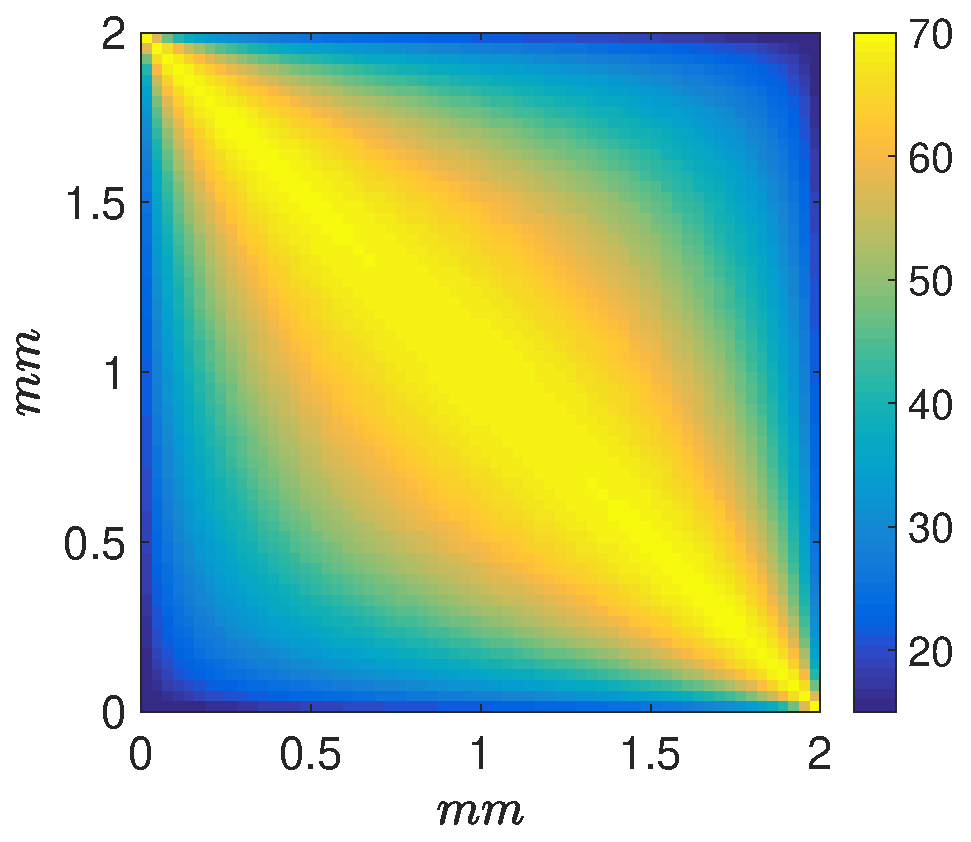
\includegraphics[width=\fwd]{figs/E110_CBFOnDifferentResolutions_plot-Ps-scaleto-none-raw.eps} 
%		& 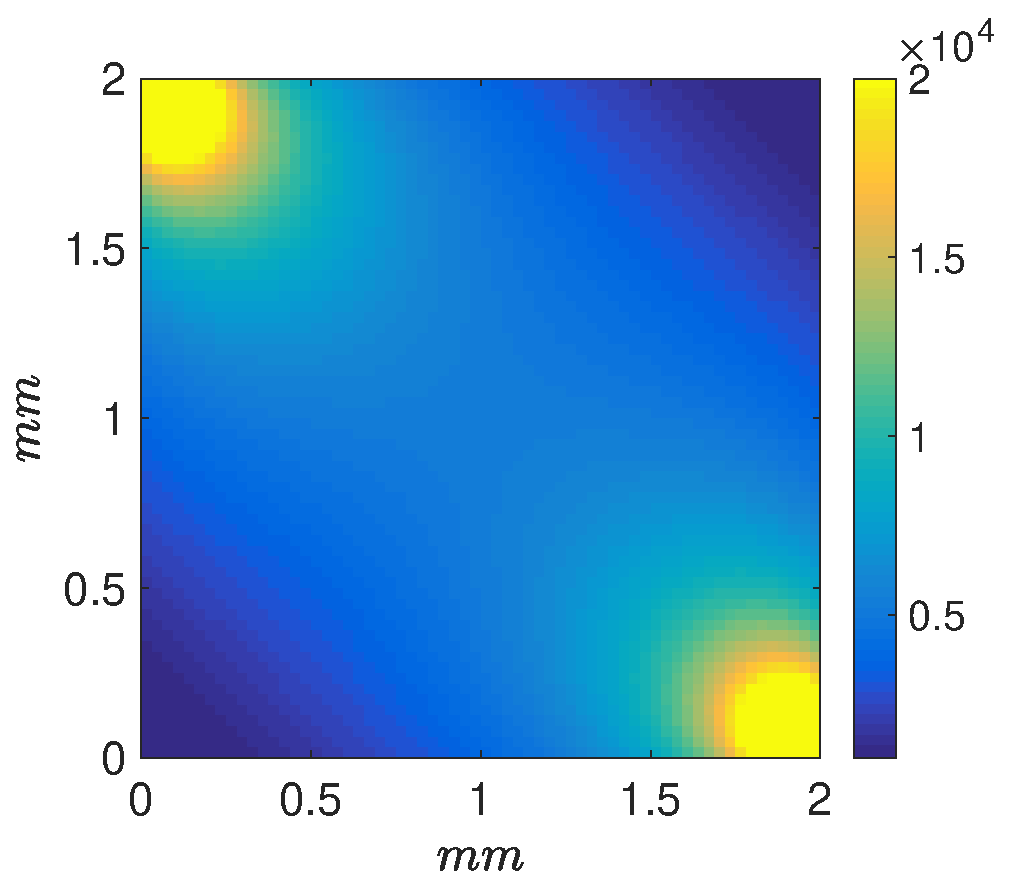
\includegraphics[width=\fwd]{figs/E110_CBFOnDifferentResolutions_plot-Pv-scaleto-none-raw.eps}
%		& 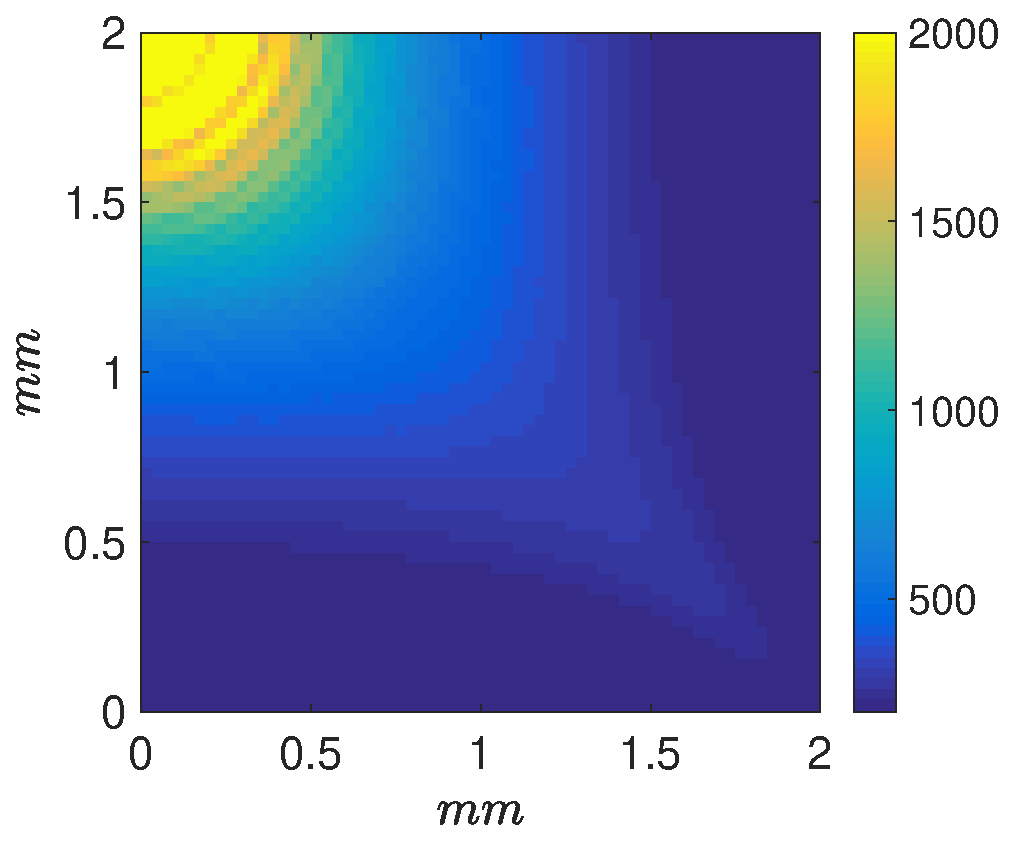
\includegraphics[width=\fwd]{figs/E110_CBFOnDifferentResolutions_plot-bSVD-scaleto-none-raw.eps}
%		& 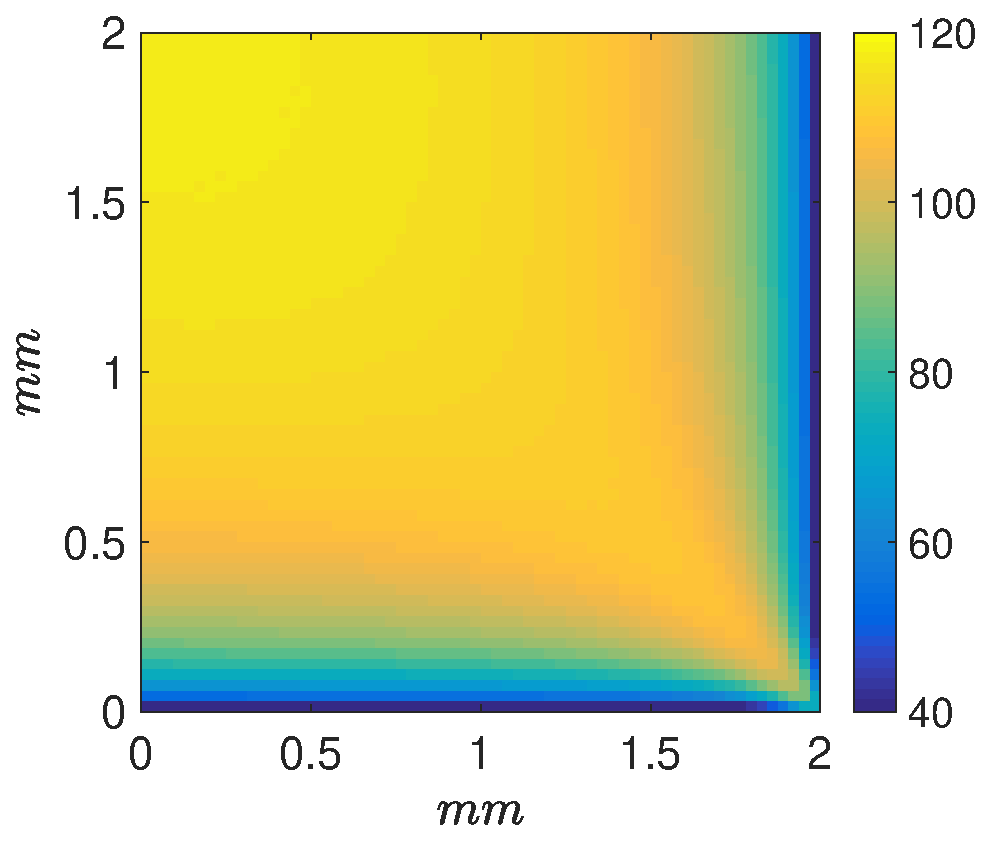
\includegraphics[width=\fwd]{figs/E110_CBFOnDifferentResolutions_plot-MS-scaleto-none-raw.eps}\\
%		(a) $P_{\mathrm{s}}(\mathbf{x})$. & (b) $P_{\mathrm{v}}(\mathbf{x})$ & (c) $P_{\mathrm{bSVD}}(\mathbf{x})$. & (d) $P_{\mathrm{MS}}(\mathbf{x})$.
%	\end{tabular}
%	\caption{Ground truth (a-b) and reconstructed (c-d) perfusion maps [\SI{}{\milli\litre\per\minute\per 100\milli\litre}] at the lowest discretization scale. The reconstructed perfusion maps have substantially varying characteristics compared to any of the two grond truth perfusion maps. (a) Global perfusion $P_{\mathrm{s}}(\mathbf{x})$ along the streamlines according to \eqref{eq:flux2perf}. (c) Local perfusion $P_{\mathrm{v}}(\mathbf{x})$ according to \eqref{eq:perflocal}. (c) Reconstructed perfusion $P_{\mathrm{bSVD}}$ according to \eqref{eq:conv}. (d) Reconstructed perfusion $P_{\mathrm{MS}}$ according to \eqref{eq:MS}.} 
%        \label{fig:perfusionmaps}
%\end{figure*}	

	%This definition most accurately reflects the physical perfusion at a given location and shows plausible perfusion values, cf. Figure~\ref{fig:flowpressureperfusion}. 
	We performed two different normalizations of the restored flow, a normalization (i) with respect to volume, and (ii) with respect to surface.  %Average flow over the entire domain $\Omega$ is denoted $\overline{F}$. 
The volume normalization (i) implies normalizing the flow to  [\SI{}{\milli\litre\per\minute\per100\milli\litre}]. A comparison of ground truth perfusion to reconstructed perfusion using volume normalization is shown in Figure \ref{fig:volnormperf}. For a voxel size corresponding to the entire ROI (voxel size = \SI{3}{\milli\meter}) the reconstructed perfusion of $P_{\mathrm{bSVD}}$ and $P_{\mathrm{MS}}$ is close to the ground truth perfusion $P_{\mathrm{s}}$ and $P_{\mathrm{v}}$. For any voxel size smaller than the entire domain the relative error increases inversely with voxel size, in particular for reconstruction by bSVD. Global perfusion $P_{\mathrm{s}}$ is not depending on voxel size.


\begin{figure}[!h]
\caption{{\bf Restored perfusion as a function of voxel size}
Comparison of restored perfusion with ground truth perfusion as a function of varying voxel size. Dotted, blue lines show average perfusion (left axis). Solid, red lines are average, relative errors (RE) of restored perfusion as compared to ground truth perfusion (right axis). (a) Global perfusion $P_{\mathrm{s}}$ is independent of discretization.  Subdivision of the domain into smaller cells leads to a substantial overestimation of perfusion for both reconstruction methods. (b) Local perfusion $P_{\mathrm{v}}$ is dependent on discretization level. A subdivision of the domain leads to substantial underestimation of perfusion when compared to $P_{\mathrm{v}}$ for both reconstruction methods.}
\label{fig:volnormperf}
\end{figure}


%    \begin{figure*}[!htb]
%    	\centering
%    	\fwd = .46\textwidth
%    	\begin{tabular}{c c}
%    		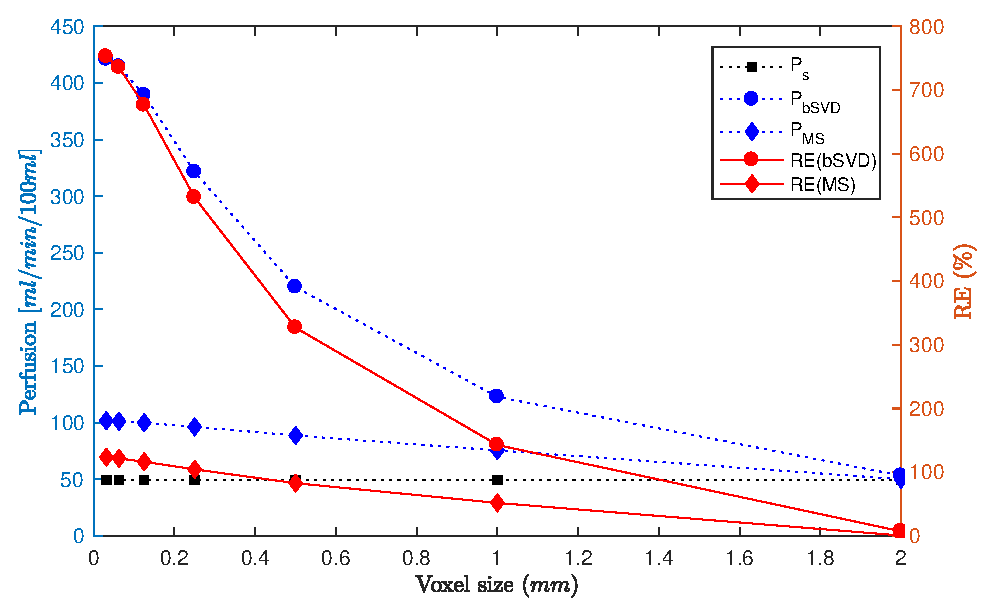
\includegraphics[width=\fwd]{figs/E110_CBFOnDifferentResolutions_plot-Ps-scaleto-none.eps} & 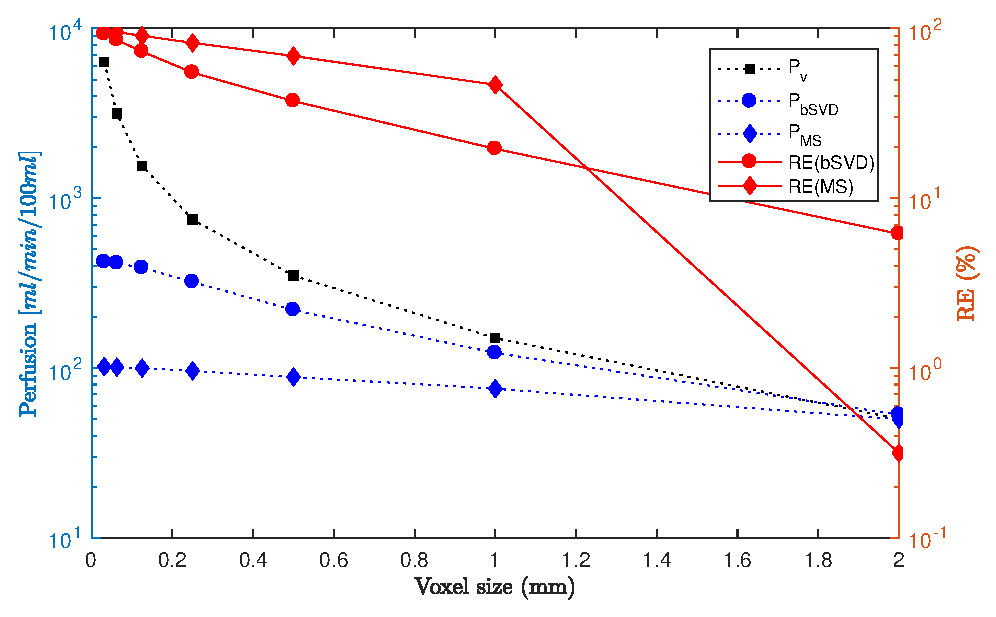
\includegraphics[width=\fwd]{figs/E110_CBFOnDifferentResolutions_plot-Pv-scaleto-none.eps}\\	
%    		(a) Comparison to global perfusion $P_{\mathrm{s}}$. & (b) Comparison to local perfusion $P_{\mathrm{v}}$. \\
%    	\end{tabular}
%    	\caption{Comparison of restored perfusion with ground truth perfusion as a function of varying voxel size. Dotted, blue lines show average perfusion (left axis). Solid, red lines are average, relative errors (RE) of restored perfusion as compared to ground truth perfusion (right axis). (a) Global perfusion $P_{\mathrm{s}}$ is independent of discretization.  Subdivision of the domain into smaller cells leads to a substantial overestimation of perfusion for both reconstruction methods. (b) Local perfusion $P_{\mathrm{v}}$ is dependent on discretization level. A subdivision of the domain leads to substantial underestimation of perfusion when compared to $P_{\mathrm{v}}$ for both reconstruction methods.}
%            \label{fig:volnormperf}
%    \end{figure*}
    
For surface normalization (ii) we first computed the absolute flow $F$ [\SI{}{\milli\litre\per\second}] of ground truth perfusion as well as reconstructed perfusion, and then normalized the flow to the surface area of the distribution volume $F/S$ (e.g. surface area of grid cell), here referred to as surface normalized flow. 
Reconstruction results of surface normalized flow is shown in Figure \ref{fig:surfnormperf}. For a voxel size corresponding to the entire ROI (voxel size = \SI{3}{\milli\meter} isotropic) the surface normalized flow of $P_{\mathrm{bSVD}}$ and $P_{\mathrm{MS}}$ is close to the ground truth. For any voxel size smaller than the entire domain the relative error increases inversely with voxel size, in particular for reconstruction by bSVD. Both global perfusion $P_{\mathrm{s}}$ and local perfusion $P_{\mathrm{v}}$ are dependent on voxel size.


\begin{figure}[!h]
\caption{{\bf Surface normalized flow.}
Comparison of surface normalized reconstructed flow [\SI{}{\milli\litre\per\minute/\milli\meter\squared}] to the ground truth as a function of varying voxel size. Dotted, blue lines show surface normalized flow (left axis). Solid, red lines are average, relative errors as compared to flow estimated from ground truth perfusion (right axis). (a) Black, dotted line with filled squares shows that surface normalized flow estimated from ground truth perfusion $P_{\mathrm{s}}$ is dependent on discretization level. Subdivision of the domain into smaller voxels leads to substantial overestimation of surface normalized flow for both reconstruction methods bSVD and MS. (b) Black, dotted line with filled squares shows that surface normalized flow estimated from local perfusion $P_{\mathrm{v}}$ is also dependent on discretization level. A further subdivision of the domain leads to substantial underestimation of the flow for both reconstruction methods bSVD and MS.}
\label{fig:surfnormperf}
\end{figure}



%    \begin{figure*}[!htb]
%    	\centering
%    	\fwd = .46\textwidth
%    	\begin{tabular}{c c}
%    		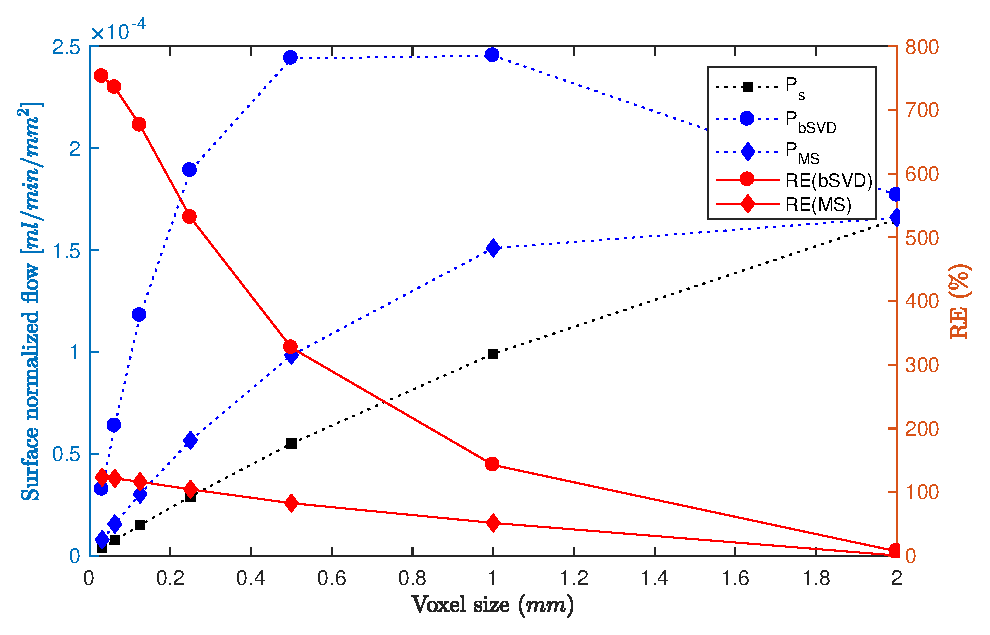
\includegraphics[width=\fwd]{figs/E110_CBFOnDifferentResolutions_plot-Ps-scaleto-S.eps} & 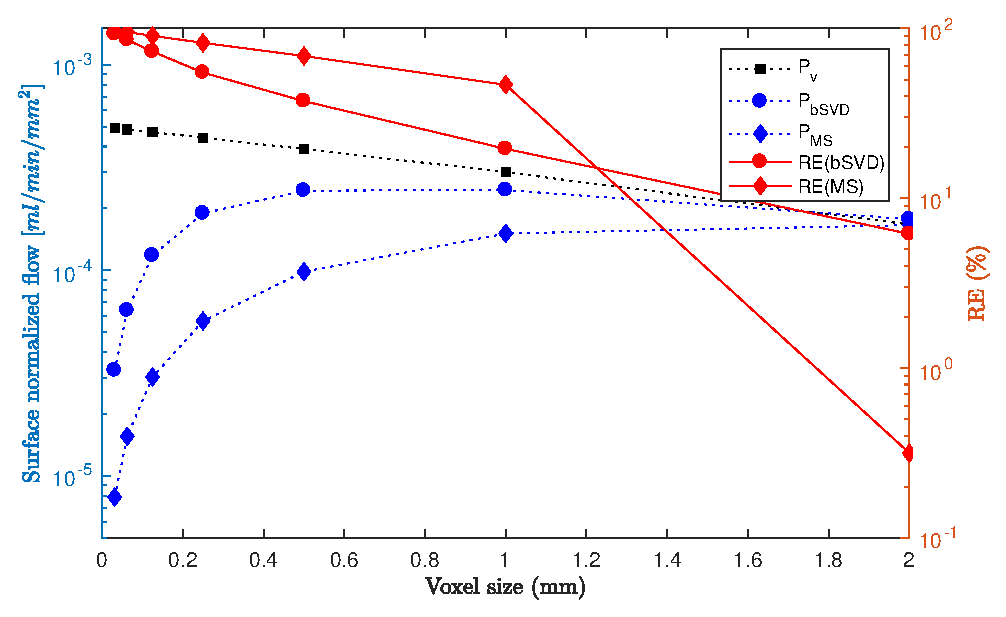
\includegraphics[width=\fwd]{figs/E110_CBFOnDifferentResolutions_plot-Pv-scaleto-S.eps}\\	
%    		(a) Comparison to global perfusion $P_{\mathrm{s}}$. & (b) Comparison to local perfusion $P_{\mathrm{v}}$.
%    	\end{tabular}
%    	\caption{Comparison of surface normalized reconstructed flow [\SI{}{\milli\litre\per\minute/\milli\meter\squared}] to the ground truth as a function of varying voxel size. Dotted, blue lines show surface normalized flow (left axis). Solid, red lines are average, relative errors as compared to flow estimated from ground truth perfusion (right axis). (a) Black, dotted line with filled squares shows that surface normalized flow estimated from ground truth perfusion $P_{\mathrm{s}}$ is dependent on discretization level. Subdivision of the domain into smaller voxels leads to substantial overestimation of surface normalized flow for both reconstruction methods bSVD and MS. (b) Black, dotted line with filled squares shows that surface normalized flow estimated from local perfusion $P_{\mathrm{v}}$ is also dependent on discretization level. A further subdivision of the domain leads to substantial underestimation of the flow for both reconstruction methods bSVD and MS.}
%            \label{fig:surfnormperf}
%    \end{figure*}

%	Results from deconvolution by traditional methods are displayed in Table~\ref{tab:resultsSim}. 
%	For the complete domain (i.e. block size $64 \times 64$), both the MS method as well as the convolution method were able to restore the ground truth perfusion of \SI{50}{\milli\litre\per\minute\per100\milli\litre} accurately with errors of $<1\%$ and $<4\%$ respectively (column header 'Entire ROI').
%	However, the errors are increasing as methods are applied to smaller blocks of the system.
%	If compared to $P_{\mathrm{v}}$, one can see that results are improving with increasing block size. 
%	Note that the block size of $(0.5,0.5)\SI{}{\milli\meter}$ is within the range of resolution available on clinical scanners today. %, and is therefore clinically interesting.
%	%\rthNote{Narrower comparison of bSVD and MS on the phantom.}	
%	Also, a clear advantage of the bSVD method as compared to MS can be observed for larger block sizes.

	%are also shown in Table~\ref{tab:resultsSim}. The errors are low, independent of block size.
	
	%--------------------------------------------------
	%--------------------------------------------------
	% Subsection: Results on Real Data
	%--------------------------------------------------
	%--------------------------------------------------	
	\subsection{Reconstruction of perfusion within real data}\label{sec:resultsrealdata}
	 Perfusion for the entire brain by averaging the concentration time curves first and then performing the bSVD yielded a perfusion of $P_{\mathrm{bSVD}}$ = \SI{24.79}{\milli\litre\per\minute\per100\milli\litre}. As a second step, voxelwise perfusion was estimated, depicted in Figure~\ref{fig:RealData}. These values yielded an average perfusion of $\overline{P}_{\mathrm{bSVD}} = $\SI{64.36}{\milli\litre\per\minute\per100\milli\litre}, corresponding to an overestimation of perfusion with $RE = 159.60\%$ compared to the value obtained for the entire brain.	


\begin{figure}[!h]
\caption{{\bf Reconstructed perfusion in real data.}
Real-data reconstruction of perfusion (see Section \ref{sec:RealData} for details). (a) AIF manually selected from the MCA. (b) One slice of restored voxelwise CBF [\si{\milli\litre\per\minute\per100\milli\litre}] from a 3D volume of interest. (c) Mean concentration time curve for the complete 3D volume of interest and the curve approximation by bSVD (rel. = relative).}
\label{fig:RealData}
\end{figure}


%	\begin{figure*}[!htb]
%		\fwd = .21\textwidth
%		\centering
%		\begin{tabular}{ccc}
%		 {\small% This file was created by matlab2tikz.
%
%The latest updates can be retrieved from
%  http://www.mathworks.com/matlabcentral/fileexchange/22022-matlab2tikz-matlab2tikz
%where you can also make suggestions and rate matlab2tikz.
%
\definecolor{mycolor1}{rgb}{0.00000,0.44700,0.74100}%
%
\begin{tikzpicture}

\begin{axis}[%
width=0.951\fwd,
height=0.75\fwd,
at={(0\fwd,0\fwd)},
scale only axis,
xmin=0,
xmax=120,
xlabel={time [s]},
ymin=0,
ymax=250,
ylabel={rel. concentration},
axis background/.style={fill=white}
]
\addplot [color=mycolor1,solid,forget plot,thick]
  table[row sep=crcr]{%
0	0\\
5	4.81948215980018\\
10	11.7249407767123\\
15	109.788176034815\\
20	221.037522824365\\
25	141.890221064755\\
30	49.1060473080009\\
35	27.7167012296253\\
40	34.5042336994668\\
45	46.9343027309933\\
50	38.6517774527303\\
55	37.0988211659761\\
60	37.9793720995833\\
65	38.8599230331905\\
70	39.7404739667976\\
75	40.6210249004048\\
80	41.501575834012\\
85	42.3663391649169\\
90	41.668129828291\\
95	40.969920491665\\
100	40.2717111550391\\
105	39.5735018184132\\
110	38.8752924817873\\
};
\end{axis}
\end{tikzpicture}%} & 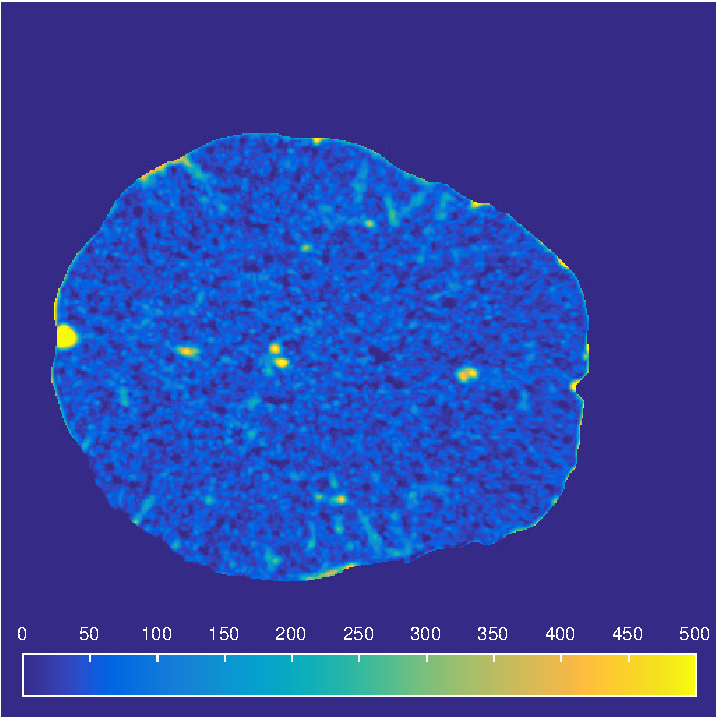
\includegraphics[width = \fwd]{./figs/real_axial160.pdf} & {\small% This file was created by matlab2tikz.
%
%The latest updates can be retrieved from
%  http://www.mathworks.com/matlabcentral/fileexchange/22022-matlab2tikz-matlab2tikz
%where you can also make suggestions and rate matlab2tikz.
%
\begin{tikzpicture}

\begin{axis}[%
width=0.951\fwd,
height=0.75\fwd,
at={(0\fwd,0\fwd)},
scale only axis,
xmin=0,
xmax=250,
xlabel={time [s]},
ymin=-2,
ymax=14,
ylabel={rel. concentration},
axis background/.style={fill=white}
]
\addplot [color=blue,solid,forget plot,thick]
  table[row sep=crcr]{%
0	0\\
5.10888888888889	3.57728482303029\\
10.2177777777778	3.8501111093967\\
15.3266666666667	5.71664126840386\\
20.4355555555556	10.3940019898786\\
25.5444444444444	13.3104878781745\\
30.6533333333333	9.7857007250912\\
35.7622222222222	7.15008816358801\\
40.8711111111111	6.69575791027159\\
45.98	7.0175162477114\\
51.0888888888889	7.11075546536433\\
56.1977777777778	7.06466948033182\\
61.3066666666667	7.08320213588359\\
66.4155555555556	7.1017347914334\\
71.5244444444444	7.12026744698453\\
76.6333333333333	7.13880010253569\\
81.7422222222222	7.15733275808708\\
86.8511111111111	7.17427131128685\\
91.96	7.03339373168847\\
97.0688888888889	6.89251615209099\\
102.177777777778	6.75163857249418\\
107.286666666667	6.61076099289567\\
112.395555555556	6.46988341329856\\
117.504444444444	0\\
122.613333333333	0\\
127.722222222222	0\\
132.831111111111	0\\
137.94	0\\
143.048888888889	0\\
148.157777777778	0\\
153.266666666667	0\\
158.375555555556	0\\
163.484444444444	0\\
168.593333333333	0\\
173.702222222222	0\\
178.811111111111	0\\
183.92	0\\
189.028888888889	0\\
194.137777777778	0\\
199.246666666667	0\\
204.355555555556	0\\
209.464444444444	0\\
214.573333333333	0\\
219.682222222222	0\\
224.791111111111	0\\
229.9	0\\
};
\addplot [color=red,solid,forget plot,thick]
  table[row sep=crcr]{%
0	0.242877310049657\\
5.10888888888889	3.27801404634268\\
10.2177777777778	4.19212893178922\\
15.3266666666667	5.35931224793637\\
20.4355555555556	10.7296350477088\\
25.5444444444444	13.0351453456191\\
30.6533333333333	9.97028747702823\\
35.7622222222222	7.06991667403901\\
40.8711111111111	6.67958740784569\\
45.98	7.10086370332965\\
51.0888888888889	7.00395379245554\\
56.1977777777778	7.14771381111792\\
61.3066666666667	7.0617592832064\\
66.4155555555556	7.04431690009689\\
71.5244444444444	7.24681150319147\\
76.6333333333333	6.97944442254963\\
81.7422222222222	7.29409620580436\\
86.8511111111111	7.12166516958014\\
91.96	6.94933713547804\\
97.0688888888889	7.14300746526767\\
102.177777777778	6.3362801703634\\
107.286666666667	7.15680159666211\\
112.395555555556	5.8535182522262\\
117.504444444444	0.612745947271016\\
122.613333333333	-0.537195282539902\\
127.722222222222	0.406490463075758\\
132.831111111111	-0.24779589623344\\
137.94	0.091958881285865\\
143.048888888889	0.0337330911498852\\
148.157777777778	-0.111471653403876\\
153.266666666667	0.136091537098496\\
158.375555555556	-0.114848569476664\\
163.484444444444	0.0641204450664707\\
168.593333333333	-0.00415036164469126\\
173.702222222222	-0.0465858173026518\\
178.811111111111	0.0758150018721239\\
183.92	-0.0795846098022592\\
189.028888888889	0.061693871067431\\
194.137777777778	-0.0308886810616511\\
199.246666666667	-0.00308806028012709\\
204.355555555556	0.0332184262864778\\
209.464444444444	-0.0574855553444383\\
214.573333333333	0.0790144471363498\\
219.682222222222	-0.104119919783985\\
224.791111111111	0.139008058015951\\
229.9	-0.186333192218881\\
};
\end{axis}
\end{tikzpicture}%} \\
%		 (a) & (b) & (c) 
%		\end{tabular}
%		\caption{Real-data reconstruction of perfusion (see Section \ref{sec:RealData} for details). (a) AIF manually selected from the MCA. (b) One slice of restored voxelwise CBF [\si{\milli\litre\per\minute\per100\milli\litre}] from a 3D volume of interest. (c) Mean concentration time curve for the complete 3D volume of interest and the curve approximation by bSVD (rel. = relative).}
%	\label{fig:RealData}
%	\end{figure*}

	

%PLOS does not support heading levels beyond the 3rd (no 4th level headings).

\section{Discussion}
\label{sec:conclusion}

It has previously been shown that perfusion reconstructed from traditional 1C models in a coupled system is discretization dependent (cfr. Figure \ref{fig:perfusion-problem}) \cite{Henkelman1990,Guibert2013,sourbron14}. As a consequence, the obtained results will strongly depend on acquisitions parameters and post-processing tools. It is unknown to which extent the pharmacokinetic modelling overestimates perfusion and whether the error is homogeneously distributed or not. Considering this, the shortcoming of existing perfusion formulations has not been sufficiently well accounted for within clinical studies \cite{Mokin16,Kickingereder15}. To clarify the potential impact of limitations seen within existing perfusion models, our main contribution of the current work is to quantify the observed error. To the best of our knowledge, such quantification has not been carried out previously.
	%To establish ground truth values, we developed a PDE based digital phantom to simulate blood flow as porous media flow within a slab of capillary tissue.
	%We have justified that the discretized PDE problem can be equivalently described as a system of coupled traditional one-compartment models.	

	% \roNote{Paragraph highlighting the relevancy for the community.}	
	Our results strongly support the usage of traditional 1C models for entire regions exclusively fed by the measured arterial input. Moreover, our results also show that if traditional models are applied only to parts of the system, the measured perfusion is overestimated (cfr. Figure \ref{fig:volnormperf}, black and blue curves). Observed error in perfusion for a characteristic voxel size typically present in modern MR scanners of $\sim$\SI{2}{\milli\meter} was found to be $\sim$$40\%$ for reconstruction by bSVD and $\sim$$20\%$ for reconstruction by MS (cfr. Figure \ref{fig:volnormperf}). The error is expected to increase in future acquisitions along with hardware and software improvements leading to higher spatial sampling.
	%These limitations are only partly known within the community, and studies reporting voxelwise perfusion maps without discussing their possible limitations are continuously published \cite{Mokin16,Kickingereder15}. 
	%Thus, a major motivation for our study is to stimulate the awareness around this topic and to push the development of more appropriate models for future applications.
		%The reason for this is that traditional models do not take into account the correct distribution volume and therefore become discretization dependent.
		
	There are at least two reasons for overestimation of perfusion in traditional 1C models. The first reason is that blood passing through a voxel without being locally delivered to the capillary tissue will contribute to artificially high perfusion values. This issue has not been accounted for in our digital model. The second reason is thoroughly described here, and relates to estimation of an incorrect distribution volume used for computing the perfusion. 
%In the presence of coupled flow between adjacent voxels, the correct distribution volume used for normalizing the absolute flow into perfusion is not known and overestimation of perfusion will occur. 
	%Using local arterial input functions is no remedy for this problem, since the resulting perfusion will depend heavily on the voxel size and overestimate the actual flow, cf. Figure~\ref{fig:perfusion-problem} and \eqref{eq:voxelcurve}.
%	In fact, in the most extreme example we measured overestimated perfusion values which were on average up to $753\%$.
	%JUST ONE NOTE: WE COULD GET ANY VALUE HERE. IF WE GO TO AN EVEN FINER SCALE THE ERROR WIL BE LARGER. WE CAN EVEN PROVE THAT THE ERROR GOES TO INF. WHEN WE APPROACH THE CONTINIOUS SCALE. 
	Overestimation of perfusion obtained within the digital phantom was also confirmed by real data experiments, where we showed local overestimation of perfusion for voxelwise estimates as compared to an averaging of concentrations for the entire volume of interest (cfr. Section \ref{sec:resultsrealdata}). 
	
	In order to demonstrate our results we introduced two definitions of voxelwise perfusion, global perfusion $P_{\mathrm{s}}$ and local perfusion $P_{\mathrm{v}}$. Local perfusion $P_{\mathrm{v}}$ is in line with \cite{Guibert2013} where the authors demonstrated a discretization dependent flow without connecting it mathematically to perfusion. Theory and examples in our work show that this definition of perfusion does not comply with the physical understanding of perfusion as a feeding arterial blood flow. The correct distribution volume is not accounted for and the obtained perfusion will be strongly overestimated compared to the actual perfusion. However, our analyses show that traditional models would restore this local flow value if the local arterial input function was selected, implying that traditional models are accurate as long as the model assumptions are not violated. The coupling between the continuous porous media model and the convolution model in Section \ref{sec:NewAndOld} demonstrates that there is no contradiction between these two models. The problematic issue of traditional models is related to physical interpretation and normalization with respect to incorrect distribution volume.

	% We have additionally analyzed, both analytically and experimentally, the impact of selecting a further upstream arterial input function.
	%Specifically, we have justified that traditional perfusion measurements based on convolution will identify the recursive impulse response function for all upstream voxels (see Section~\ref{sec:NewAndOld}). 


	Global perfusion $P_{\mathrm{s}}$ models perfusion along the streamlines and most accurately reflects the physical notion of volume flow within the correct distribution volume according to mathematical definitions. We showed that $P_{\mathrm{s}}$ is independent of discretization (cfr. Figure \ref{fig:volnormperf}), $P_{\mathrm{s}}$ is a constant quantity along the streamline, and scales with streamline length and geometry according to \eqref{eq:flux2perf}.
	%The usage of $P_{\mathrm{s}}$ for reconstruction of perfusion in real data might as well be challenging as the entire geometry and microscopical flow patterns would have to be known to track the streamlines. 
	For our purpose, the concept of $P_{\mathrm{s}}$ was useful as a realistic ground truth in order to clarify the definition of perfusion as a flow that must be normalized along the entire capillary length, where the blood undergoes a transition from arterial to venous blood. Estimation of $P_{\mathrm{s}}$ in real applications is practically difficult due to the unknown microstructure and fluid flux, and the development of new field models for perfusion is therefore highly demanded in line with multicompartment models suggested in \cite{sourbron14,Michler2013}. 
	
	% However, geometrical complexity and lack of detailed information about microscopical capillary structure justifies that traditional models cannot recover this perfusion. 
	%For future developments of field models, multi compartment models as suggested in \cite{sourbron14} might be more applicable, where the perfusion was suggested as the non-zero divergence of the arterial flux.

It was previously suggested to normalize the flow by surface instead of volume \cite{Guibert2013}. However, our experiments suggest that a surface normalization is nevertheless discretization dependent, and traditional 1C models are not able to restore this type of perfusion, neither for global, nor for local perfusion (cfr. Figure \ref{fig:surfnormperf}, blue and black lines).
%The reason why the authors in  \cite{Guibert2013} found that surface-normalized flow is discretization independent is can arise from the 
%\rthNote{Elaborated on relationship of continuous and discrete model.}

%There are at least two reasons for the discrepancy between recovered and actual perfusion in our numerical experiments. First, w
We have shown there is a global error directly scaling with smaller voxel sizes (cfr. Figure \ref{fig:volnormperf}). A comparison between individual scans with otherwise equal acquisition parameters and post-processing chains should ideally adjust for the global error in the interpretation of absolute perfusion values. As such, voxelwise maps of perfusion could still be of high clinical value as the main goal is a comparison of perfusion between patients or between repeated scans of individuals. However, particular care should be undertaken in the case of comparing perfusion data of various resolution. Multicenter or retrospective studies are particularly susceptible to this situation where data collected from various sources are different with respect to hardware, resolution and post-processing tools that can affect the discretization level. Future study design should account for this limitation and special care should be undertaken to ensure equal level of discretization in perfusion estimates. 

In addition to the observed global error we also observed inhomogeneous reconstruction errors within the capillary system. This becomes clear in Figure \ref{fig:perfusionmaps} where the reconstructed perfusion maps $P_{\mathrm{bSVD}}$ and $P_{\mathrm{MS}}$ are strongly unlike the ground truth perfusion maps of $P_{\mathrm{s}}$ and $P_{\mathrm{v}}$. This inhomogeneity leads to locally inaccurate estimates of perfusion within a patch, even if the global average value within the patch were correct. 
%The reason for this discrepancy is dispersion of the AIF within the capillary system, not accounted for in traditional 1C models. 
In analyses of voxelwise perfusion with high resolution the local error can become large within each capillary patch.
 
Regarding the CBV estimates, estimation of blood volume is stable, and varying voxel size had little impact on the results. These results are in agreement with the analyses in Section \ref{sec:CBV} supporting the usage of \eqref{eq:CBV} for computing voxelwise CBV with high accuracy for any voxel size.
	


\section{Conclusion}

Our experiments confirm that traditional 1C models for perfusion perform well if they are applied to the entire domain.
	However, when they are applied to fractions within a coupled domain, perfusion becomes scale dependent.
	We quantified substantial and increasing reconstruction errors of perfusion as a function of smaller voxel size, and we also found similar effects in real data. The observed reconstruction error for a resolution found in clinical MR scanners was between $\sim$$20\%$ to $\sim$$40\%$. The reason for the observed errors is not numerical instabilities in the deconvolution but rather that traditional 1C models will not account for correct distribution volume within smaller fractions of the region of interest. As a consequence, interpretation of absolute perfusion for the purpose of diagnosis and disease monitoring must be undertaken with care, and comparison of perfusion values from individual dynamic data sets with different resolution is not recommended. 
	%The scale-dependency is expected to become more pronounced in future as imaging hardware is constantly improving in spatial resolution.
	%We expect to find overestimation also in pathological tissue, and recommend to be take this effect into consideration for clinical evaluation of such data. 

%\section{Supporting information}

%\section{Acknowledgments}
%Cras egestas velit mauris, eu mollis turpis pellentesque sit amet. Interdum et malesuada fames ac ante ipsum primis in faucibus. Nam id pretium nisi. Sed ac quam id nisi malesuada congue. Sed interdum aliquet augue, at pellentesque quam rhoncus vitae.

%
%\fwd = .4\textwidth
%\fht = .1\textheight	
%\begin{figure*}[p]
%	{
%	\small
%	% \begin{tabular}{p{\fwd} p{\fwd}}
%	\begin{tabular}{c c}
%		% This file was created by matlab2tikz.
%
%The latest updates can be retrieved from
%  http://www.mathworks.com/matlabcentral/fileexchange/22022-matlab2tikz-matlab2tikz
%where you can also make suggestions and rate matlab2tikz.
%
\definecolor{mycolor1}{rgb}{0.00000,0.44700,0.74100}%
\definecolor{mycolor2}{rgb}{0.85000,0.32500,0.09800}%
%
\begin{tikzpicture}

\begin{axis}[%
width=0.951\fwd,
height=0.75\fht,
at={(0\fwd,0\fwd)},
scale only axis,
xmin=0,
xmax=40,
xlabel={time [s]},
ymin=0,
ymax=2.5e-07,
ylabel={$C$ $\text{[mmol/mm}^\text{3}\text{]}$},
axis background/.style={fill=white},
legend style={legend cell align=left,align=left,draw=white!15!black}
]
\addplot [color=mycolor1,solid,very thick]
  table[row sep=crcr]{%
0	0\\
0.4	0\\
0.8	0\\
1.2	0\\
1.6	0\\
2	5.62373487759478e-11\\
2.4	1.09810271021085e-09\\
2.8	6.76053034703798e-09\\
3.2	2.13478347753626e-08\\
3.6	4.56056649657982e-08\\
4	7.67693039618778e-08\\
4.4	1.10760368816952e-07\\
4.8	1.43746597983364e-07\\
5.2	1.72821999990385e-07\\
5.6	1.96160012105964e-07\\
6	2.12907090713985e-07\\
6.4	2.22973323725445e-07\\
6.8	2.26804741960865e-07\\
7.2	2.25178885025859e-07\\
7.6	2.19040032343215e-07\\
8	2.09376955393214e-07\\
8.4	1.97139176006753e-07\\
8.8	1.83184972235038e-07\\
9.2	1.6825381701405e-07\\
9.6	1.5295649926078e-07\\
10	1.3777726549853e-07\\
10.4	1.23083485704354e-07\\
10.8	1.09139475580703e-07\\
11.2	9.61220627108628e-08\\
11.6	8.41362598740187e-08\\
12	7.32300105168483e-08\\
12.4	6.34074188236187e-08\\
12.8	5.46401838538925e-08\\
13.2	4.68771886140848e-08\\
13.6	4.00523095626387e-08\\
14	3.4090617904463e-08\\
14.4	2.89131601344388e-08\\
14.8	2.44405364930844e-08\\
15.2	2.05954798314946e-08\\
15.6	1.73046252038486e-08\\
16	1.44996421001143e-08\\
16.4	1.21178699857602e-08\\
16.8	1.01025854633713e-08\\
17.2	8.40299542178553e-09\\
17.6	6.97404198461131e-09\\
18	5.77607935091924e-09\\
18.4	4.77447355834304e-09\\
18.8	3.93916172160292e-09\\
19.2	3.24419737926786e-09\\
19.6	2.66730266166506e-09\\
20	2.18943870651418e-09\\
20.4	1.79440465920876e-09\\
20.8	1.46846847064005e-09\\
21.2	1.20003289411346e-09\\
21.6	9.79336326007395e-10\\
22	7.98187748378252e-10\\
22.4	6.49733970754416e-10\\
22.8	5.28256526672998e-10\\
23.2	4.28995952016572e-10\\
23.6	3.48000282397405e-10\\
24	2.81995444125054e-10\\
24.4	2.28274651883307e-10\\
24.8	1.84604584011355e-10\\
25.2	1.49146036254608e-10\\
25.6	1.20387064957272e-10\\
26	9.70868785116934e-11\\
26.4	7.82288318545415e-11\\
26.8	6.29812300119354e-11\\
27.2	5.06646643040334e-11\\
27.6	4.07249116439323e-11\\
28	3.27104678363883e-11\\
28.4	2.62539803586422e-11\\
28.8	2.10569311946487e-11\\
29.2	1.68770204325555e-11\\
29.6	1.35178038053597e-11\\
30	1.0820183236205e-11\\
30.4	8.65544366249652e-12\\
30.8	6.91955310729552e-12\\
31.2	5.5285112362483e-12\\
31.6	4.41455486319452e-12\\
32	3.52306811834916e-12\\
32.4	2.81007005409287e-12\\
32.8	2.2401727856489e-12\\
33.2	1.78492607969931e-12\\
33.6	1.42147458549083e-12\\
34	1.13147177733343e-12\\
34.4	0\\
34.8	0\\
35.2	0\\
35.6	0\\
36	0\\
36.4	0\\
36.8	0\\
37.2	0\\
37.6	0\\
38	0\\
38.4	0\\
38.8	0\\
39.2	0\\
39.6	0\\
};
\addlegendentry{Convolution};

\addplot [color=mycolor2,dashed,very thick]
  table[row sep=crcr]{%
0	0\\
0.4	0\\
0.8	0\\
1.2	0\\
1.6	0\\
2	5.3279568073074e-11\\
2.4	1.07821521955639e-09\\
2.8	6.71290754043026e-09\\
3.2	2.12564956013061e-08\\
3.6	4.54228810841506e-08\\
4	7.64315332182225e-08\\
4.4	1.10213523840219e-07\\
4.8	1.42958770768866e-07\\
5.2	1.71785826132747e-07\\
5.6	1.94889508729946e-07\\
6	2.11432221500284e-07\\
6.4	2.21334146149828e-07\\
6.8	2.25046160287466e-07\\
7.2	2.23346407714781e-07\\
7.6	2.17176667633836e-07\\
8	2.07521150089304e-07\\
8.4	1.95323644243314e-07\\
8.8	1.81436224500391e-07\\
9.2	1.66592199968555e-07\\
9.6	1.51396589797636e-07\\
10	1.3632847936435e-07\\
10.4	1.21750799207446e-07\\
10.8	1.07924182119412e-07\\
11.2	9.50225094085739e-08\\
11.6	8.31485298722586e-08\\
12	7.2348531031234e-08\\
12.4	6.26254832899861e-08\\
12.8	5.39503908539349e-08\\
13.2	4.62717953679953e-08\\
13.6	3.95235135517039e-08\\
14	3.36307690244454e-08\\
14.4	2.85149175130422e-08\\
14.8	2.40969765219252e-08\\
15.2	2.03001649700339e-08\\
15.6	1.70516423039829e-08\\
16	1.4283615166056e-08\\
16.4	1.19339562230449e-08\\
16.8	9.94645645486966e-09\\
17.2	8.27081040255549e-09\\
17.6	6.86241431416851e-09\\
18	5.68204011719055e-09\\
18.4	4.6954337247387e-09\\
18.8	3.87287421966553e-09\\
19.2	3.18872072804604e-09\\
19.6	2.62096602035629e-09\\
20	2.15080978220791e-09\\
20.4	1.76225980427895e-09\\
20.8	1.44176580276721e-09\\
21.2	1.17788797530892e-09\\
21.6	9.61000531233148e-10\\
22	7.83029147436785e-10\\
22.4	6.37220457950388e-10\\
22.8	5.1794117711445e-10\\
23.2	4.20504195487211e-10\\
23.6	3.41018904827157e-10\\
24	2.76263049750932e-10\\
24.4	2.23573527582697e-10\\
24.8	1.80753733306562e-10\\
25.2	1.45995250370183e-10\\
25.6	1.17811903729239e-10\\
26	9.4984407302507e-11\\
26.4	7.65140460587736e-11\\
26.8	6.15840282729948e-11\\
27.2	4.95273231768238e-11\\
27.6	3.97999619242864e-11\\
28	3.19589252105288e-11\\
28.4	2.56438694661132e-11\\
28.8	2.05620562202835e-11\\
29.2	1.64759471844691e-11\\
29.6	1.31930121953556e-11\\
30	1.05573697632337e-11\\
30.4	8.44294196192858e-12\\
30.8	6.74785807138353e-12\\
31.2	5.38988595036491e-12\\
31.6	4.30270767561291e-12\\
32	3.43288752398976e-12\\
32.4	2.73740677349094e-12\\
32.8	2.18166182862043e-12\\
33.2	1.73784050750156e-12\\
33.6	1.38360654329319e-12\\
34	1.10103495034139e-12\\
34.4	0\\
34.8	0\\
35.2	0\\
35.6	0\\
36	0\\
36.4	0\\
36.8	0\\
37.2	0\\
37.6	0\\
38	0\\
38.4	0\\
38.8	0\\
39.2	0\\
39.6	0\\
};
\addlegendentry{PDE};

\end{axis}
\end{tikzpicture}% & \input{./figs/IDecVSIAna.tikz}\\
%	\end{tabular}
%	}
%	\caption*{}
%	\label{fig:VoxelCompFIG}
%\end{figure*}
%\clearpage
%
%	\begin{figure*}[p]
%	    \centering
%	    \begin{overpic}[scale=0.3]{figs/perfusion-problem.eps}
%	    	\put(10,70){\color{black}$F_0$}
%			\put(48,70){\color{black}$F_0$}
%			\put(84,70){\color{black}$\Delta F_0$}
%			\put(10,33){\color{black}$2V$}
%			\put(49,20){\color{black}$V$}
%			\put(49,45){\color{black}$V$}
%			\put(91,42){\color{black}$\Delta V$}
%		\end{overpic}
%	    \caption*{}
%	    \label{fig:perfusion-problemFIG}
%	\end{figure*}
%\clearpage
%
%\begin{figure*}[p]
%	\centering
%	\fwd = .23\textwidth
%	\begin{tabular}{c c c c}
%		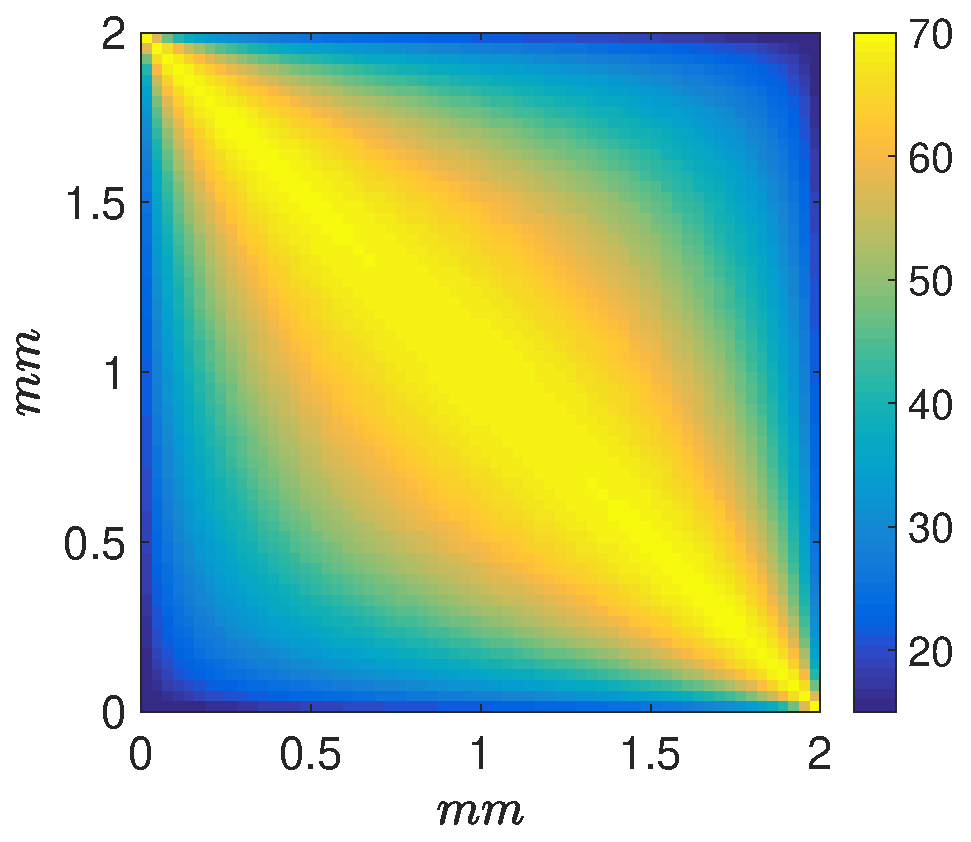
\includegraphics[width=\fwd]{figs/E110_CBFOnDifferentResolutions_plot-Ps-scaleto-none-raw.eps} 
%		& 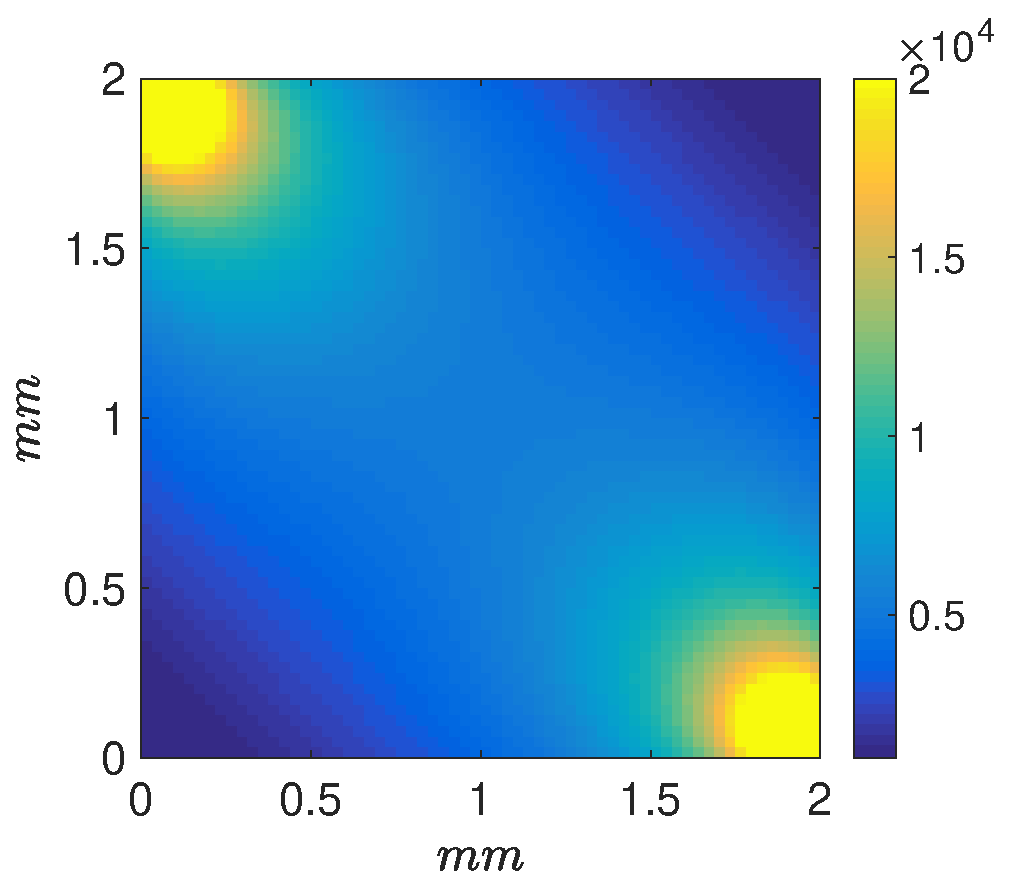
\includegraphics[width=\fwd]{figs/E110_CBFOnDifferentResolutions_plot-Pv-scaleto-none-raw.eps}
%		& 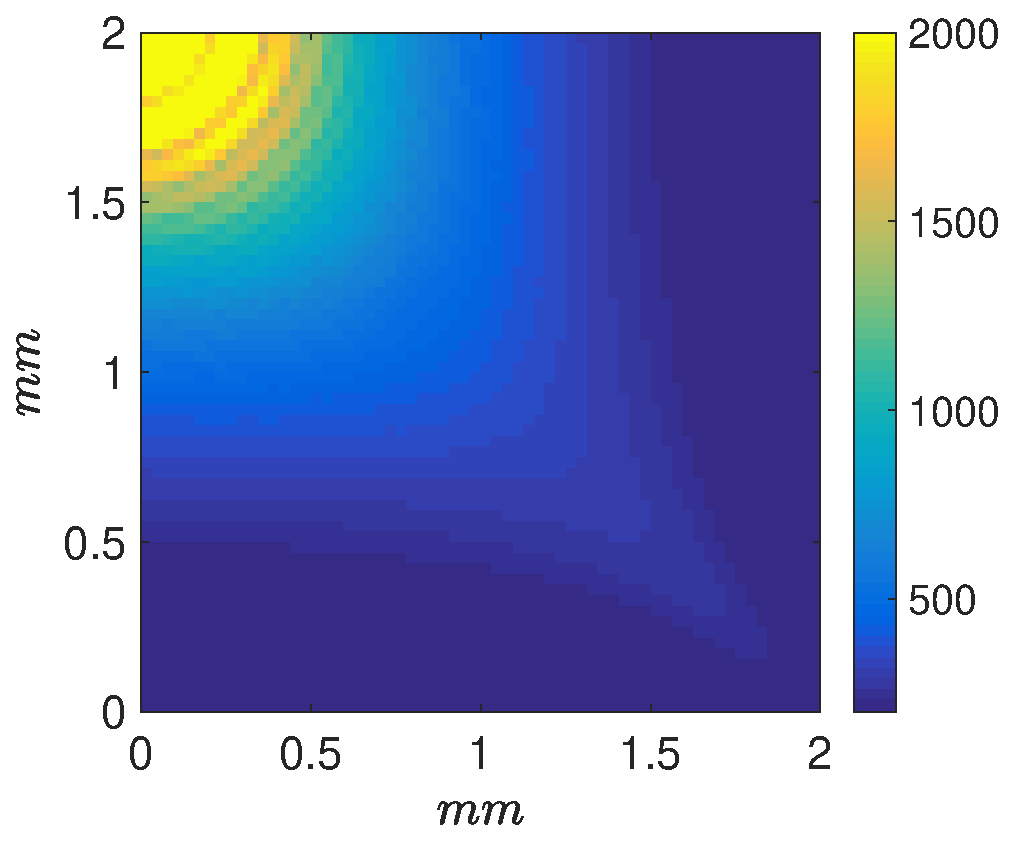
\includegraphics[width=\fwd]{figs/E110_CBFOnDifferentResolutions_plot-bSVD-scaleto-none-raw.eps}
%		& 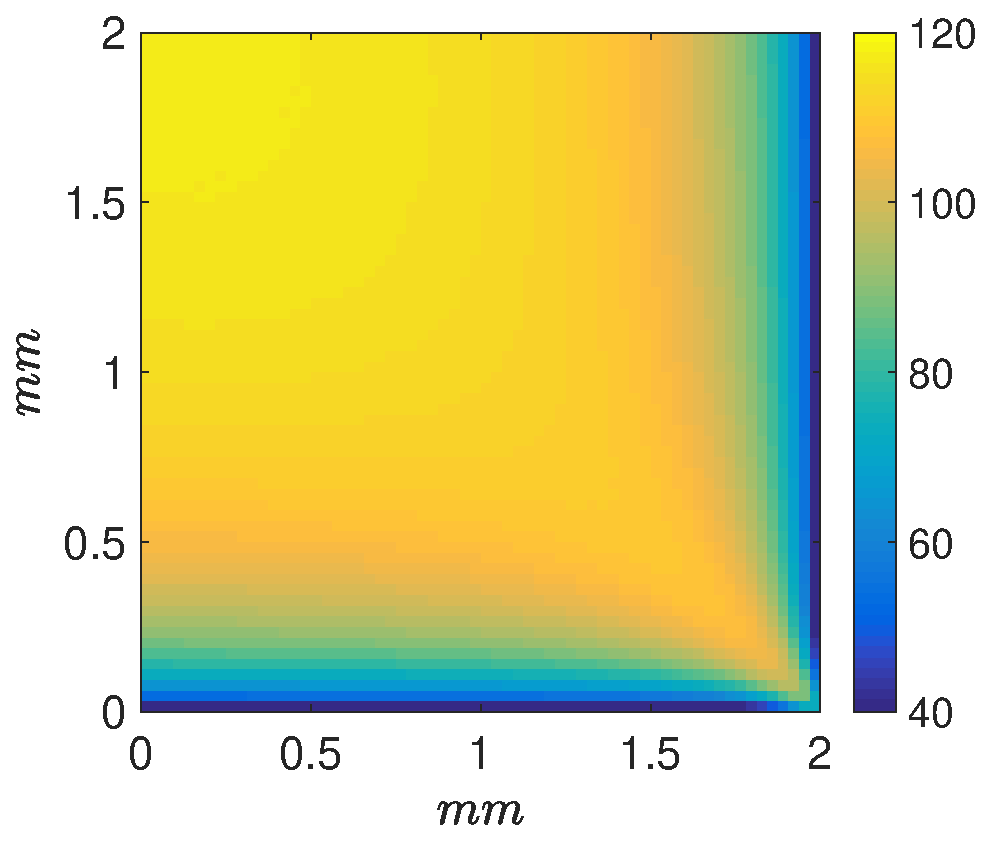
\includegraphics[width=\fwd]{figs/E110_CBFOnDifferentResolutions_plot-MS-scaleto-none-raw.eps}\\
%		(a) $P_{\mathrm{s}}(\mathbf{x})$. & (b) $P_{\mathrm{v}}(\mathbf{x})$ & (c) $P_{\mathrm{bSVD}}(\mathbf{x})$. & (d) $P_{\mathrm{MS}}(\mathbf{x})$.
%	\end{tabular}
%	\caption*{} 
%        \label{fig:perfusionmapsFIG}
%\end{figure*}	
%\clearpage
%
%    \begin{figure*}[p]
%    	\centering
%    	\fwd = .46\textwidth
%    	\begin{tabular}{c c}
%    		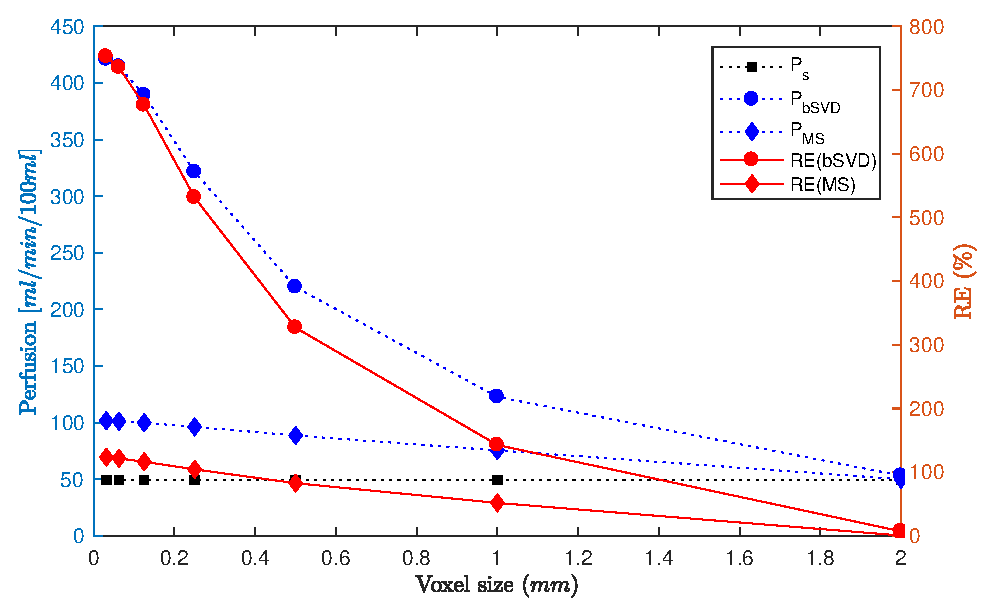
\includegraphics[width=\fwd]{figs/E110_CBFOnDifferentResolutions_plot-Ps-scaleto-none.eps} & 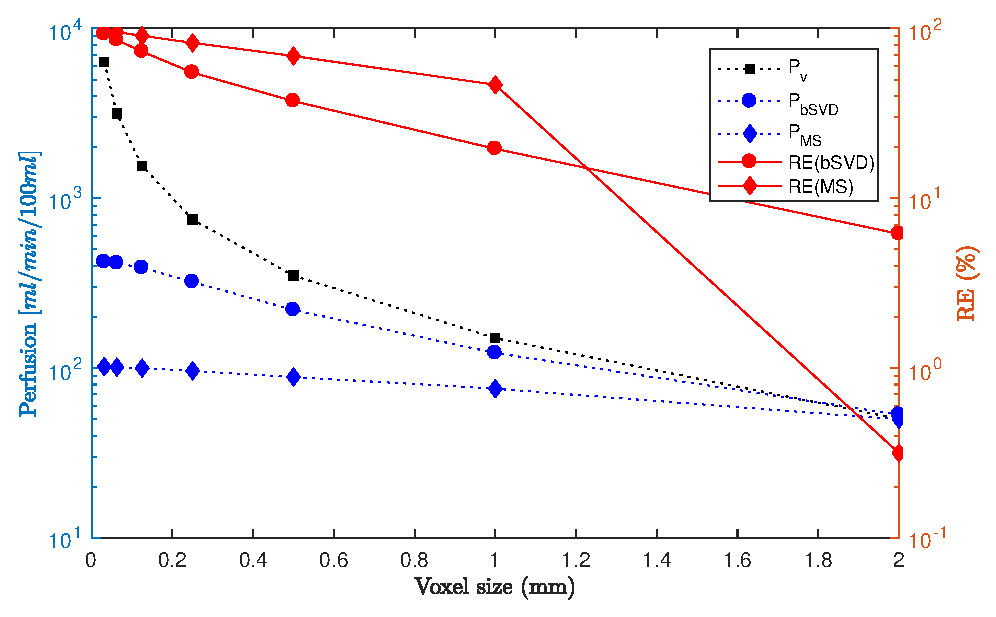
\includegraphics[width=\fwd]{figs/E110_CBFOnDifferentResolutions_plot-Pv-scaleto-none.eps}\\	
%    		(a) Comparison to global perfusion $P_{\mathrm{s}}$. & (b) Comparison to local perfusion $P_{\mathrm{v}}$. \\
%    	\end{tabular}
%    	\caption*{}
%            \label{fig:volnormperfFIG}
%    \end{figure*}
%\clearpage
%
%    \begin{figure*}[p]
%    	\centering
%    	\fwd = .46\textwidth
%    	\begin{tabular}{c c}
%    		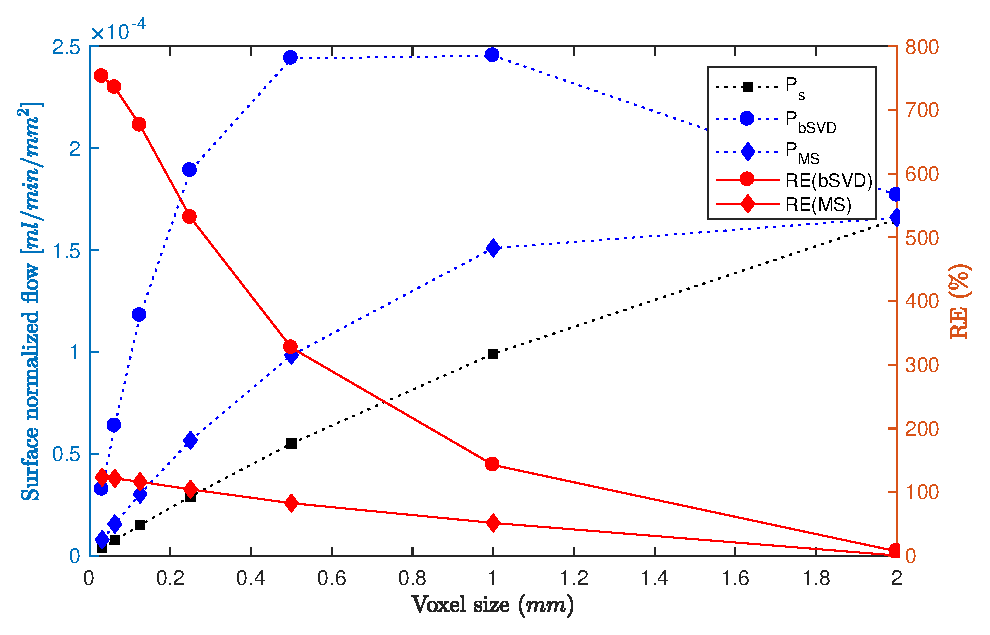
\includegraphics[width=\fwd]{figs/E110_CBFOnDifferentResolutions_plot-Ps-scaleto-S.eps} & 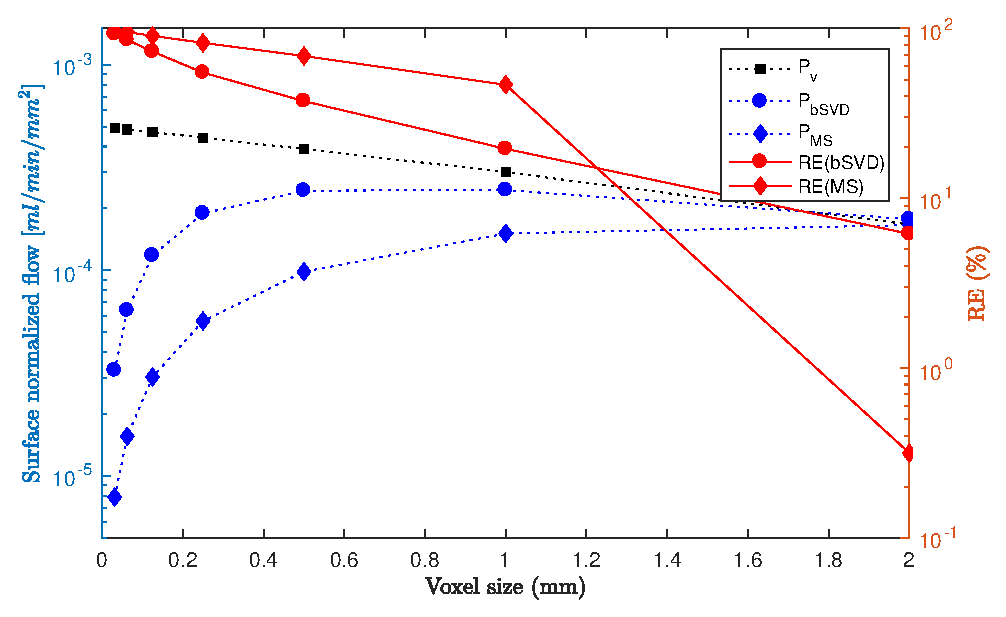
\includegraphics[width=\fwd]{figs/E110_CBFOnDifferentResolutions_plot-Pv-scaleto-S.eps}\\	
%    		(a) Comparison to global perfusion $P_{\mathrm{s}}$. & (b) Comparison to local perfusion $P_{\mathrm{v}}$.
%    	\end{tabular}
%    	\caption*{}
%            \label{fig:surfnormperfFIG}
%    \end{figure*}
%\clearpage
%
%	\begin{figure*}[p]
%		\fwd = .21\textwidth
%		\centering
%		\begin{tabular}{ccc}
%		 {\small% This file was created by matlab2tikz.
%
%The latest updates can be retrieved from
%  http://www.mathworks.com/matlabcentral/fileexchange/22022-matlab2tikz-matlab2tikz
%where you can also make suggestions and rate matlab2tikz.
%
\definecolor{mycolor1}{rgb}{0.00000,0.44700,0.74100}%
%
\begin{tikzpicture}

\begin{axis}[%
width=0.951\fwd,
height=0.75\fwd,
at={(0\fwd,0\fwd)},
scale only axis,
xmin=0,
xmax=120,
xlabel={time [s]},
ymin=0,
ymax=250,
ylabel={rel. concentration},
axis background/.style={fill=white}
]
\addplot [color=mycolor1,solid,forget plot,thick]
  table[row sep=crcr]{%
0	0\\
5	4.81948215980018\\
10	11.7249407767123\\
15	109.788176034815\\
20	221.037522824365\\
25	141.890221064755\\
30	49.1060473080009\\
35	27.7167012296253\\
40	34.5042336994668\\
45	46.9343027309933\\
50	38.6517774527303\\
55	37.0988211659761\\
60	37.9793720995833\\
65	38.8599230331905\\
70	39.7404739667976\\
75	40.6210249004048\\
80	41.501575834012\\
85	42.3663391649169\\
90	41.668129828291\\
95	40.969920491665\\
100	40.2717111550391\\
105	39.5735018184132\\
110	38.8752924817873\\
};
\end{axis}
\end{tikzpicture}%} & 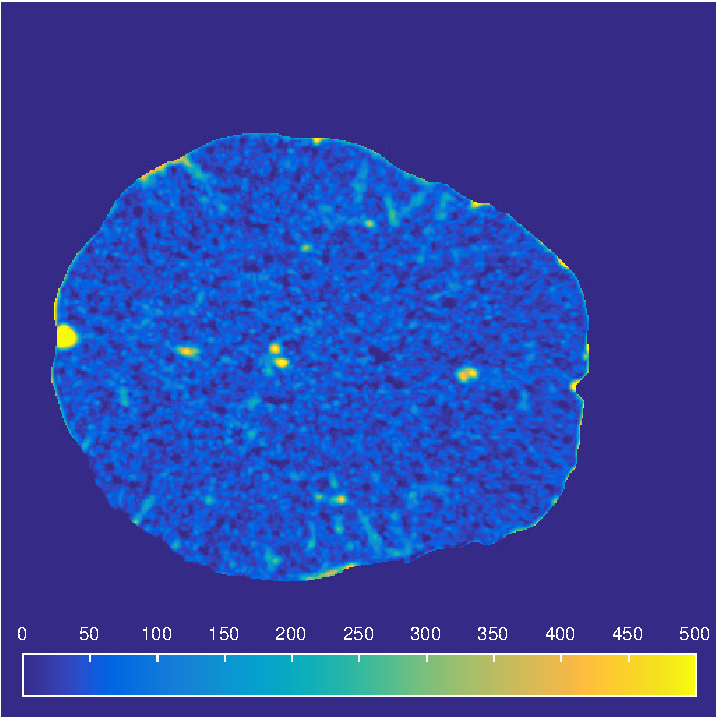
\includegraphics[width = \fwd]{./figs/real_axial160.pdf} & {\small% This file was created by matlab2tikz.
%
%The latest updates can be retrieved from
%  http://www.mathworks.com/matlabcentral/fileexchange/22022-matlab2tikz-matlab2tikz
%where you can also make suggestions and rate matlab2tikz.
%
\begin{tikzpicture}

\begin{axis}[%
width=0.951\fwd,
height=0.75\fwd,
at={(0\fwd,0\fwd)},
scale only axis,
xmin=0,
xmax=250,
xlabel={time [s]},
ymin=-2,
ymax=14,
ylabel={rel. concentration},
axis background/.style={fill=white}
]
\addplot [color=blue,solid,forget plot,thick]
  table[row sep=crcr]{%
0	0\\
5.10888888888889	3.57728482303029\\
10.2177777777778	3.8501111093967\\
15.3266666666667	5.71664126840386\\
20.4355555555556	10.3940019898786\\
25.5444444444444	13.3104878781745\\
30.6533333333333	9.7857007250912\\
35.7622222222222	7.15008816358801\\
40.8711111111111	6.69575791027159\\
45.98	7.0175162477114\\
51.0888888888889	7.11075546536433\\
56.1977777777778	7.06466948033182\\
61.3066666666667	7.08320213588359\\
66.4155555555556	7.1017347914334\\
71.5244444444444	7.12026744698453\\
76.6333333333333	7.13880010253569\\
81.7422222222222	7.15733275808708\\
86.8511111111111	7.17427131128685\\
91.96	7.03339373168847\\
97.0688888888889	6.89251615209099\\
102.177777777778	6.75163857249418\\
107.286666666667	6.61076099289567\\
112.395555555556	6.46988341329856\\
117.504444444444	0\\
122.613333333333	0\\
127.722222222222	0\\
132.831111111111	0\\
137.94	0\\
143.048888888889	0\\
148.157777777778	0\\
153.266666666667	0\\
158.375555555556	0\\
163.484444444444	0\\
168.593333333333	0\\
173.702222222222	0\\
178.811111111111	0\\
183.92	0\\
189.028888888889	0\\
194.137777777778	0\\
199.246666666667	0\\
204.355555555556	0\\
209.464444444444	0\\
214.573333333333	0\\
219.682222222222	0\\
224.791111111111	0\\
229.9	0\\
};
\addplot [color=red,solid,forget plot,thick]
  table[row sep=crcr]{%
0	0.242877310049657\\
5.10888888888889	3.27801404634268\\
10.2177777777778	4.19212893178922\\
15.3266666666667	5.35931224793637\\
20.4355555555556	10.7296350477088\\
25.5444444444444	13.0351453456191\\
30.6533333333333	9.97028747702823\\
35.7622222222222	7.06991667403901\\
40.8711111111111	6.67958740784569\\
45.98	7.10086370332965\\
51.0888888888889	7.00395379245554\\
56.1977777777778	7.14771381111792\\
61.3066666666667	7.0617592832064\\
66.4155555555556	7.04431690009689\\
71.5244444444444	7.24681150319147\\
76.6333333333333	6.97944442254963\\
81.7422222222222	7.29409620580436\\
86.8511111111111	7.12166516958014\\
91.96	6.94933713547804\\
97.0688888888889	7.14300746526767\\
102.177777777778	6.3362801703634\\
107.286666666667	7.15680159666211\\
112.395555555556	5.8535182522262\\
117.504444444444	0.612745947271016\\
122.613333333333	-0.537195282539902\\
127.722222222222	0.406490463075758\\
132.831111111111	-0.24779589623344\\
137.94	0.091958881285865\\
143.048888888889	0.0337330911498852\\
148.157777777778	-0.111471653403876\\
153.266666666667	0.136091537098496\\
158.375555555556	-0.114848569476664\\
163.484444444444	0.0641204450664707\\
168.593333333333	-0.00415036164469126\\
173.702222222222	-0.0465858173026518\\
178.811111111111	0.0758150018721239\\
183.92	-0.0795846098022592\\
189.028888888889	0.061693871067431\\
194.137777777778	-0.0308886810616511\\
199.246666666667	-0.00308806028012709\\
204.355555555556	0.0332184262864778\\
209.464444444444	-0.0574855553444383\\
214.573333333333	0.0790144471363498\\
219.682222222222	-0.104119919783985\\
224.791111111111	0.139008058015951\\
229.9	-0.186333192218881\\
};
\end{axis}
\end{tikzpicture}%} \\
%		 (a) & (b) & (c) 
%		\end{tabular}
%		\caption*{}
%	\label{fig:RealDataFIG}
%	\end{figure*}
%
\nolinenumbers

% Either type in your references using
% \begin{thebibliography}{}
% \bibitem{}
% Text
% \end{thebibliography}
%
% or
%
% Compile your BiBTeX database using our plos2015.bst
% style file and paste the contents of your .bbl file
% here. See http://journals.plos.org/plosone/s/latex for 
% step-by-step instructions.
% 
\bibliography{./bibliography}
\bibliographystyle{plos2015} 


\end{document}

